\documentclass[openany]{book}

\usepackage[DIV=9]{typearea}

\makeatletter
\if@twoside % commands below work only for twoside option of \documentclass
    \newlength{\textblockoffset}
    \setlength{\textblockoffset}{12mm}
    \addtolength{\hoffset}{\textblockoffset}
    \addtolength{\evensidemargin}{-2.0\textblockoffset}
\fi
\makeatother

\usepackage[english]{babel}
\usepackage[utf8]{inputenc} % For spanish characters
\usepackage[T1]{fontenc} % For special characters
\usepackage{times} 
\usepackage{emptypage} 
\usepackage{pgfplots}
\usepackage{graphicx}
\usepackage{color}
\usepackage{float, multirow, rotating}
\usepackage[autolanguage]{numprint}
\usepackage{xspace}
\usepackage{mathtools, amsmath, amsthm, amssymb, enumerate}
\usepackage{hyphenat}
\usepackage{caption, subcaption}
\usepackage{url}
\usepackage{multirow} 
\usepackage{rotating}
\usepackage[ruled, vlined, linesnumbered, resetcount]{algorithm2e}
\usepackage{appendix}
\usepackage{units}
\usepackage{setspace}
\usepackage{fancyhdr}
\usepackage{lipsum}
\usepackage{csquotes}
\usepackage{subcaption}   % for subfigure
\usepackage{float}        % for [H] (exact placement)
\usepackage{placeins}     % for \FloatBarrier
\usepackage{needspace}
% Optionally (nice tables):
\usepackage{booktabs}
\usepackage{longtable}
\usepackage[
  backend=biber,
  style=ieee,
  citestyle=ieee,
  sorting=none,
  defernumbers=true,
  maxbibnames=99,
  maxcitenames=2,
  giveninits=true,
  isbn=false,
  doi=true,
  url=false,
  eprint=false
]{biblatex}
% Añadir espacio entre párrafos y quitar sangría
\usepackage{parskip}

% Hacer que el título sea un enlace si hay DOI (Opcional pero recomendado)
\newbibmacro{string+doi}[1]{%
  \iffieldundef{doi}{#1}{\href{https://doi.org/\thefield{doi}}{#1}}}
\DeclareFieldFormat{title}{\usebibmacro{string+doi}{\mkbibemph{#1}}}
\DeclareFieldFormat[article,inproceedings,incollection]{title}%
    {\usebibmacro{string+doi}{\mkbibquote{#1}}}

\addto\captionsspanish{}

% Redefine the name of the list of tables
\addto\captionsspanish{
  \renewcommand{\listtablename}{List of Tables}
}

\DeclareNameAlias{sortname}{first-last}
\setlength{\bibitemsep}{\baselineskip}

\newcommand{\image}[4]{
\begin{figure}[H]
\centering
\includegraphics[width=#2\linewidth,height=0.45\textheight,keepaspectratio]{./images/#1}
\caption{#3}
\label{#4}
\end{figure}
}

\newcommand{\requirement}[3]{
\begin{table}[h!]
\centering
\input{#1}
\caption{#2}
\label{#3}
\end{table}
}

\addto\captionsspanish{\renewcommand{\tablename}{Table}}

\addbibresource{references.bib}

\let\parencite\cite

\usepackage{hyperref}
\hypersetup{
   colorlinks,
   linktoc=all, 
   linkcolor=blue, 
   citecolor=blue,
   urlcolor=blue
}

\DefineBibliographyStrings{english}{%
  backrefpage = {page},% originally "cited on page"
  backrefpages = {pages},% originally "cited on pages"
}

\sloppy
\raggedbottom
\addtocontents{toc}{\protect\thispagestyle{empty}}

% Custom command to add keywords
\newenvironment{keywords}[1]{
  \list{}{\advance\topsep by 0.35cm\relax\small
  \leftmargin=0.7cm
  \labelsep=0.1cm
  \listparindent=0cm
  \itemindent\listparindent
  \rightmargin\leftmargin}\item[\hskip\labelsep\bfseries#1:]}
  {\endlist}

\definecolor{maincolor}{RGB}{240,127,9} 

\pagestyle{plain}
\fancyhf{} % Clears the default header and footer

\fancypagestyle{plain}{
  \fancyhf{}
  \fancyhead{}
  \fancyfoot[RO]{\rule{\textwidth}{0.2pt} \\ \hfill \textbf{\textcolor{maincolor}{COMPUTER SCIENCE DEGREE}}}
  \fancyfoot[LE]{\rule{\textwidth}{0.2pt} \\ \textbf{\textcolor{maincolor}{FINAL DEGREE PROJECT}} | Universidad Francisco de Vitoria \hfill \thepage}
  \renewcommand{\headrulewidth}{0pt}
  \renewcommand{\footrulewidth}{0pt}
}
% Redefine the plain page style for the first page of chapters
\fancypagestyle{fancy}{
  \fancyhf{}
  \fancyhead{}
  \fancyfoot[RO]{\rule{\textwidth}{0.1pt} \\ \hfill \textbf{\textcolor{maincolor}{COMPUTER SCIENCE DEGREE}}}
  \fancyfoot[LE]{\rule{\textwidth}{0.1pt} \\ \textbf{\textcolor{maincolor}{FINAL DEGREE PROJECT}} | Universidad Francisco de Vitoria \hfill \thepage}
  \renewcommand{\headrulewidth}{0pt}
  \renewcommand{\footrulewidth}{0pt}
}


\setcounter{tocdepth}{1}
\newcommand{\myname}{Francisco Sandoval Hern{\'a}ndez}
\newcommand{\tutor}{Mois{\'e}s Mart{\'i}nez Muñ{\'o}z}
\newcommand{\subject}{Final Degree Project (FDP)}
\newcommand{\mykeywords}{Sign Language Recognition, Artificial Intelligence, Deep Neural Networks, Computer Vision, Hand Landmarks}
\newcommand{\mykeywordses}{reconocimiento de lengua de signos, inteligencia artificial, redes neuronales profundas, visi{\'o}n por computador, puntos clave de la mano}
\newcommand{\mytitle}{Word-Level American Sign Language Recognition from Hand Landmarks}

\hypersetup{pdfauthor={\myname{}},%
            pdftitle={\mytitle{}},%
            pdfsubject={\subject{}},%
            pdfkeywords={\mykeywords{}},%
            pdfproducer={LaTeX},%
            pdfcreator={pdfLaTeX}}

\begin{document}

\renewcommand{\thepage}{\roman{page}}

\pagestyle{empty}

\begin{center}
    
\includegraphics[width=6cm]{./images/logo.jpg}
\end{center}

\vspace{1.25cm}
\begin{center}
    {\LARGE UNIVERSIDAD FRANCISCO DE VITORIA}
\end{center}

\vspace{0.15cm}
\begin{center}
    {\large \bf  ESCUELA  POLIT{\'E}CNICA SUPERIOR}
\end{center}

\vspace{0.15cm}
\begin{center}
    {\large \bf COMPUTER SCIENCE DEGREE}
\end{center}

\vspace{2.5cm}
\begin{center}
    {\Large FINAL DEGREE PROJECT}
\end{center}

\vspace{0.15cm}
\begin{center}
    {\Large RESEARCH TRACK}
\end{center}

\vspace{1.0cm}

\begin{center}
    \begin{minipage}{0.9\textwidth}
        \centering
        {\Huge\bfseries\textcolor{maincolor}{\mytitlecover{}}}
    \end{minipage}
\end{center}

\vspace{4.0cm}

\begin{flushright}
    {\normalsize \myname{}}
\end{flushright}

\vspace{0.25cm}
\begin{flushright}
    {\normalsize Tutor: \tutor{}}
\end{flushright}

\newpage{}

\phantom{}

\newpage{}

\newcolumntype{P}[1]{>{\centering\arraybackslash}m{#1}}

\begin{center}
    \textbf{CALIFICACI{\'O}N DEL PROYECTO DE FIN DE GRADO}
\end{center}

\vspace{1cm}

\begin{center}
    \begin{tabular}{|P{3cm}|P{9cm}|}
        \hline
        \textbf{CUALITATIVA:\vspace{0.5cm}} & \\ \hline
        \textbf{NUMÉRICA:\vspace{0.5cm}}    & \\ \hline
    \end{tabular}
\end{center}

\vspace{1cm}

\begin{center}
    \begin{tabular}{|P{6cm}|P{6cm}|}
        \hline
        \textbf{Conforme Presidente:} & \textbf{Conforme Secretario:} \\ \hline
                                      &                               \\[2cm] \hline
        Fdo.:                         & Fdo.:                         \\[2cm] \hline
    \end{tabular}
\end{center}

\vspace{1cm}

\begin{center}
    \begin{tabular}{|P{3.8cm}|P{3.8cm}|P{3.8cm}|}
        \hline
        \textbf{Conforme Vocal:} & \textbf{Conforme Vocal:} & \textbf{Conforme Vocal:} \\ \hline
                                 &                          &                          \\[2cm] \hline
        Fdo.:                    & Fdo.:                    & Fdo.:                    \\[2cm] \hline
    \end{tabular}
\end{center}

\vspace{1cm}

\begin{center}
    Lugar y fecha: Pozuelo de Alarcón, a \_\_\_\_ de \_\_\_\_\_\_\_\_\_\_\_\_\_ de 2026
\end{center}

\newpage{}

\pagestyle{empty}

\chapter*{Acknowledgements}

First and foremost, I would like to thank my parents, Francisco Sandoval and Gabriela Hernández,
for their unconditional support and for always believing in me, even in moments when I found it
difficult to believe in myself. Thank you for giving me the opportunity to study what I truly
wanted, in the place where I wanted to do it, and for supporting my decisions throughout this
journey.I know these four years have not always been easy, and that standing by me during them has
required patience, understanding, and love. Your support has been a constant source of strength,
and I am deeply grateful for everything you have done for me.

I would also like to thank my sister, Gabriela Sandoval. Even though we may not always see eye to
eye, I know that you have always been there for me, and I am truly grateful for that. You have
helped me more than you may realize, especially in helping me navigate difficult moments with Mum
and Dad, and in sometimes taking on situations that were really mine to face. Thank you for your
patience, your support, and for standing by me in your own way.

I would also like to thank my other brother, my dog Pepe, for literally always being there. During
all those times when we were the only ones at home, and during the late night study sessions when
you were the only one still awake, you stayed by my side. Your quiet company made many difficult
days feel a little lighter.

I would also like to give special thanks to my \tutor{} for choosing to supervise my Final Degree
Project. It is no secret that I may not always be the easiest student, and perhaps even less so
when it comes to tutoring a project. Knowing this, I am especially grateful that you still decided
to take me on.

Your guidance, patience, and understanding have been invaluable throughout this process. Even in
moments when the project felt overwhelming or almost impossible, you helped me move forward and
find my way. Thank you for helping me complete a project that I am truly proud of.

Lastly I would like to thank the rest of my family and friends, even though they might think they
where not really that helpful, just knowing that they where there for me, and that they where
willing to help me when I needed it, made it easier to get through this journey.
\chapter*{Abstract}

Sign language recognition is an important accessibility challenge, as it can help reduce communication barriers between deaf or hard-of-hearing signers and non-signing people. This project develops and evaluates a research prototype for word-level American Sign Language recognition from short video clips. The
final approach extracts 21 three-dimensional hand landmarks per frame with MediaPipe Hands, normalises the resulting sequences, and classifies ASL glosses using a bidirectional GRU with a Temporal Attention mechanism. The work also documents the methodological evolution from YOLO-based hand detection and static
letter recognition toward landmark-based temporal modelling, where the main challenge lies in representing sign motion rather than localising hands. The system was validated through experiments on WLASL and MS-ASL, including architecture comparison, sequence-length analysis, cross-dataset evaluation, and
vocabulary scaling. Results indicate promising performance for reduced vocabularies and reproducible behaviour across datasets, but also clear limitations as the number of classes increases. The landmark representation provides a privacy-friendly abstraction, although the prototype remains a research system
rather than a production-ready translator.

\begin{keywords}{Keywords}
  \mykeywords{}
\end{keywords}

\chapter*{Resumen}

\lipsum[1-2]

\begin{keywords}{Palabras claves}
  \mykeywordses{}
\end{keywords}

\tableofcontents{}
\listoffigures{}
\listoftables{}
\cleardoublepage
\chapter*{List of Acronyms}
\addcontentsline{toc}{chapter}{List of Acronyms}

\begingroup
    \renewcommand{\arraystretch}{1.25}
    \begin{longtable}{@{}p{3.0cm}p{10.5cm}@{}}
        \toprule
        \textbf{Acronym} & \textbf{Meaning}                                        \\
        \midrule
        \endfirsthead
        \toprule
        \textbf{Acronym} & \textbf{Meaning}                                        \\
        \midrule
        \endhead
        AI               & Artificial Intelligence                                 \\
        API              & Application Programming Interface                       \\
        ASL              & American Sign Language                                  \\
        AWS              & Amazon Web Services                                     \\
        BBox             & Bounding Box                                            \\
        BiGRU            & Bidirectional Gated Recurrent Unit                      \\
        BPTT             & Backpropagation Through Time                            \\
        CEC              & Constant Error Carousel                                 \\
        CNN              & Convolutional Neural Network                            \\
        CRISP-DM         & Cross-Industry Standard Process For Data Mining         \\
        CSV              & Comma-Separated Values                                  \\
        CUDA             & Compute Unified Device Architecture                     \\
        CV               & Cross-Validation                                        \\
        FDP              & Final Degree Project                                    \\
        FR               & Functional Requirement                                  \\
        GPU              & Graphics Processing Unit                                \\
        GRU              & Gated Recurrent Unit                                    \\
        HTTP             & Hypertext Transfer Protocol                             \\
        IoU              & Intersection Over Union                                 \\
        JSON             & JavaScript Object Notation                              \\
        JSONL            & JavaScript Object Notation Lines                        \\
        LTS              & Long-Term Support                                       \\
        LSTM             & Long Short-Term Memory                                  \\
        mAP              & Mean Average Precision                                  \\
        ML               & Machine Learning                                        \\
        MNIST            & Modified National Institute Of Standards And Technology \\
        MS-ASL           & Microsoft American Sign Language                        \\
        NFR              & Non-Functional Requirement                              \\
        OpenCV           & Open Source Computer Vision Library                     \\
        REST             & Representational State Transfer                         \\
        RGB              & Red Green Blue                                          \\
        RNN              & Recurrent Neural Network                                \\
        RQ               & Research Question                                       \\
        SLR              & Sign Language Recognition                               \\
        SO               & Specific Objective                                      \\
        SSDLite          & Single Shot Detector Lite                               \\
        TTA              & Test-Time Augmentation                                  \\
        UFV              & Universidad Francisco De Vitoria                        \\
        URL              & Uniform Resource Locator                                \\
        VRAM             & Video Random-Access Memory                              \\
        WLASL            & Word-Level American Sign Language                       \\
        XML              & Extensible Markup Language                              \\
        YAML             & Human-Readable Data Serialisation Language              \\
        YOLO             & You Only Look Once                                      \\
        \bottomrule
    \end{longtable}
\endgroup

% Verification check:
% Acronyms used in the document body whose full meaning is not explicitly introduced in the surrounding body text and should be verified manually:
% API, AWS, BBox, CRISP-DM, CSV, CUDA, GPU, HTTP, IoU, JSON, JSONL, LTS, mAP, ML, MNIST, OpenCV, REST, RGB, SSDLite, UFV, URL, VRAM, XML, YAML, YOLO.

%%\listofalgorithms{}

\pagestyle{fancy}

\cleardoublepage
\setcounter{page}{1}% Start page number with 2
\renewcommand{\thepage}{\arabic{page}}% Arabic numerals for page counter

\chapter{Introduction}
\setcounter{section}{0}

Sign Language Recognition (SLR) represents a highly interdisciplinary paradigm at the intersection
of digital accessibility, computer vision, and temporal sequence modelling, focused on capturing
fully-fledged, sophisticated natural languages where semantic meaning is conveyed simultaneously
rather than sequentially through distinct grammatical, syntactic, and visual-spatial structures.

\section{Problem description}

This project studies American Sign Language (ASL) recognition as an accessibility-oriented research
problem. Unlike static image classification, sign recognition is inherently temporal: a single
frame may show the handshape and approximate location of a sign, but it cannot represent the
direction of movement, the order of articulatory changes or the rhythm of execution. The sign must
therefore be interpreted from the ordered relationship between frames.

This temporal nature makes the problem substantially different from conventional object or gesture
recognition. Two signs may share a similar hand configuration in an individual frame, while
differing in trajectory, speed, orientation changes or relative hand position over time. In
addition, real videos introduce variability in signer appearance, camera viewpoint, lighting
conditions, signing style and execution speed. A recognition system must therefore learn not only
visual patterns, but also how those patterns evolve across a short sequence.

The task addressed in this work is isolated word recognition. The system receives a short video
clip and must assign it to a word gloss, that is, a written label used to annotate a sign. This
formulation is more limited than continuous sign language translation, where complete sentences,
grammar, co-articulation and broader linguistic context must be considered. However, isolated
recognition still captures a central challenge of SLR: identifying a meaningful visual unit from
motion and hand articulation.

\section{Research scope and approach}

The central research question of this work is whether compact visual representations can provide
enough information for temporal models to classify short ASL video clips into word glosses. The
project evaluates different neural architectures under reproducible experimental conditions, with
the objective of identifying a configuration that balances accuracy and computational cost. The
work does not aim to replace professional interpreters or to deliver a production-ready translator.

The experimental work is grounded on public ASL datasets, mainly WLASL \cite{li2020wlasl} and
MS-ASL \cite{joze2019msasl}. A mobile and server-based runtime prototype is also developed as a
proof of concept, although the main scientific contribution is the experimental evaluation of the
recognition approach rather than the deployment of an assistive product.

\section{Outline}

The remainder of the work is organised as follows:
\begin{itemize}
    \item Chapter 2 reviews the State of the Art, providing the theoretical foundation in computer
          vision and deep learning required for this work. It examines convolutional neural
          networks and pose estimation, specifically MediaPipe Hands, before addressing temporal
          modelling through recurrent networks, Long Short-Term Memory (LSTM) layers, Gated
          Recurrent Unit (GRU) layers, Transformers and attention mechanisms. The chapter also
          evaluates previous research in SLR to establish the context for the current approach.
    \item Chapter 3 defines the main objective, the specific objectives, and the validation methods
          used to determine whether each objective has been achieved.
    \item Chapter 4 outlines the methodology and project work plan. It details the iterative,
          experiment-driven approach adopted throughout development and delineates the main project
          phases. Finally, it addresses the technical resources and constraints that influenced the
          scope and design of the project.
    \item Chapter 5 presents the technical development and system architecture. It provides a
          rigorous account of the data preprocessing pipeline and the experimental framework
          established for training and evaluation. The chapter concludes with a description of a
          functional proof of concept, demonstrating a real-time implementation through a mobile
          app and a FastAPI-based inference server.
    \item Chapter 6 reports the experimental evaluation. It includes an architecture comparison and
          sequence-length analysis, followed by validation on the WLASL30 and MS-ASL50 datasets.
          The chapter also addresses cross-dataset validation, vocabulary scaling and the
          qualitative validation design, and concludes with a critical discussion of the main
          limitations observed during experimentation.
    \item Chapter 7 analyses the ethical implications and social impact of the project, structured
          around the Google Artificial Intelligence Principles and ethical framework. It provides a
          critical examination of accessibility, privacy and algorithmic bias, while addressing the
          requirements for responsible deployment and the importance of reproducibility. Finally,
          it evaluates the broader social value of assistive technologies through these ethical
          guidelines.
    \item Chapter 8 reflects on the academic journey at Universidad Francisco de Vitoria and
          relates the project to the competences developed during the degree.
    \item Chapter 9 presents the conclusions and future work, summarising the main findings, the
          limitations of the current prototype, and possible directions for extending the research.
\end{itemize}
\chapter{State of the Art}
\label{ch:sota}

This chapter reviews the technical foundations that support this project. It begins by exploring
the evolution of Artificial Intelligence (AI), tracing the shift from early symbolic AI based on
rules and logic techniques to modern sub-symbolic AI based on learning techniques. It then
introduces the core components of Deep Neural Networks (DNNs) that drive this sub-symbolic
paradigm, including feature extraction architectures, sequence and parallel processing
architectures, and attention mechanisms. Finally, the chapter contextualises these technologies by
reviewing previous work in Sign Language Recognition (SLR) and the main datasets used in American
Sign Language (ASL) research.

\section{From Symbolic to Subsymbolic AI}

Early AI systems were symbolic, representing knowledge through explicit logic and predefined rule
sets. They solved problems by applying human-authored rules, often organised as conditional
decision trees. While this paradigm flourished within constrained environments, it proved
inadequate for perception tasks, such as computer vision and speech, due to the inherent noise,
ambiguity, and high-dimensionality of real-world data. This phenomenon, termed the "knowledge
acquisition bottleneck", implies that as task complexity scales, the maintenance of handcrafted
rule bases becomes untenable.

In the context of sign language, symbolic approaches could encode basic gesture prototypes, but
they failed to capture the nuanced articulatory variation found across signers, camera angles and
execution speeds. A fixed rule for a hand shape may describe an idealised sign, yet the observed
motion in video changes with signer anatomy, partial occlusion, lighting and the temporal rhythm of
the execution. These sources of variation make exhaustive symbolic description impractical.

Subsymbolic AI addresses the same class of problems through statistical learning. Instead of
hard-coding expert rules for every possible case, a learning system estimates parameters from
examples. This transition was driven by advances in neural networks and statistical learning
theory, culminating in deep learning methods that learn hierarchical features directly from raw
inputs \cite{lecun2015deeplearning}. By treating perception as a high-dimensional optimisation
problem, these systems reduce the noise and ambiguity that previously led to the knowledge
acquisition bottleneck.

In the SLR domain, this transition mirrors the evolution of the field: moving away from attempts to
define a perfect hand-shape rules and towards architectures that extract latent features from raw
video data. Consequently, the burden of feature engineering shifts from the human expert to the
learning algorithm, allowing for a more fluid and robust interpretation of manual dynamics that
aligns with the success seen in modern speech recognition and object detection frameworks.

\section{Deep Neural Networks}
\label{sec:dnn}

A Deep Neural Network (DNN) is a parameterised function composed of layered computational
structures designed to map inputs to specific outputs. Each layer receives an input vector, applies
a linear transformation and passes the result through a non-linear activation function. A DNN
stacks several such layers sequentially, allowing the model to compose simple, low-level
mathematical transformations into progressively more abstract, high-level representations.
Figure~\ref{fig:dnn_basic} shows this structure as a mapping from input features to an output
prediction through hidden layers.

\begin{figure}[H]
    \centering
    \begin{tikzpicture}[
            scale=0.95,
            every node/.style={font=\small},
            neuron/.style={draw=black,circle,minimum size=0.78cm,inner sep=0pt,line width=0.45pt},
            input neuron/.style={neuron,fill=black!5},
            hidden neuron/.style={neuron,fill=black!12},
            output neuron/.style={neuron,fill=black!20},
            connection/.style={->,black!55,line width=0.35pt},
            highlighted connection/.style={->,black,line width=0.65pt}
        ]
        \node[input neuron] (i1) at (0,2) {$x_1$};
        \node[input neuron] (i2) at (0,1) {$x_2$};
        \node[input neuron] (i3) at (0,0) {$x_3$};
        \node[hidden neuron] (h11) at (2,2.5) {};
        \node[hidden neuron] (h12) at (2,1.5) {$\sigma$};
        \node[hidden neuron] (h13) at (2,0.5) {};
        \node[hidden neuron] (h14) at (2,-0.5) {};
        \node[hidden neuron] (h21) at (4,2) {};
        \node[hidden neuron] (h22) at (4,1) {$\sigma$};
        \node[hidden neuron] (h23) at (4,0) {};
        \node[output neuron] (o1) at (6,1.5) {$\hat{y}_1$};
        \node[output neuron] (o2) at (6,0.5) {$\hat{y}_2$};

        \foreach \i in {i1,i2,i3}
        \foreach \h in {h11,h12,h13,h14}
        \draw[connection] (\i) -- (\h);
        \foreach \h in {h11,h12,h13,h14}
        \foreach \g in {h21,h22,h23}
        \draw[connection] (\h) -- (\g);
        \foreach \g in {h21,h22,h23}
        \foreach \o in {o1,o2}
        \draw[connection] (\g) -- (\o);

        \draw[highlighted connection] (i2) -- node[above,sloped,font=\scriptsize,fill=white,inner sep=1pt] {$w_{ij}$} (h12);
        \draw[highlighted connection] (h12) -- node[above,sloped,font=\scriptsize,fill=white,inner sep=1pt] {$\sigma(\cdot)$} (h22);

        \node at (0,-1.35) {Input layer};
        \node at (2,-1.35) {Hidden layer};
        \node at (4,-1.35) {Hidden layer};
        \node at (6,-1.35) {Output layer};
    \end{tikzpicture}
    \caption{Basic DNN structure. Inputs are transformed through hidden layers into an output prediction. Source: self-created.}
    \label{fig:dnn_basic}
\end{figure}

For a layer $l$, the computation can be written as:
\begin{equation}
    \mathbf{h}^{(l)} = \sigma\left(\mathbf{W}^{(l)}\mathbf{h}^{(l-1)} + \mathbf{b}^{(l)}\right)
\end{equation}
where $\mathbf{W}^{(l)}$ contains the learned weights, $\mathbf{b}^{(l)}$ is the bias vector and
$\sigma$ is the activation function. The Rectified Linear Unit (ReLU), defined as
$\text{ReLU}(x)=\max(0,x)$, is a common activation because it introduces non-linearity while keeping
the computation simple. The output layer depends on the task: classification layers estimate class
probabilities, whereas regression layers estimate continuous quantities such as coordinates.

Training adjusts the parameters $\theta=\{\mathbf{W},\mathbf{b}\}$ so that the function
$f_{\theta}$ maps inputs to the desired targets. The model computes a prediction, compares it with
the ground truth through a loss function and updates the parameters by gradient-based optimisation.
In this sense, a DNN is not a list of explicit rules but an optimised function approximator.

This formulation explains the link between DNNs and feature extraction. Intermediate layers do not
only transform the data numerically; they also produce representations that make the target task
easier. In Computer Vision, these representations may correspond to edges, textures, object parts
or pose coordinates. Feature extraction therefore denotes the process of converting raw
observations into informative variables that a later classifier or sequence model can use.

\section{Feature Extraction Architectures}
\label{sec:feature_extraction_architectures}

Feature extraction architectures convert video frames into representations that preserve relevant
visual information while reducing irrelevant variation. In SLR, two families are especially
important. Pixel-based techniques operate directly on image tensors, where each pixel stores colour
or intensity values. Pose estimation techniques first detect anatomical points and then represent
the signer through coordinates. The distinction matters because it determines whether the model
learns from appearance information or from a geometric abstraction of the body and hands.

\subsection{Pixel-Based Techniques}

A digital image can be represented as a tensor $\mathbf{x}\in\mathbb{R}^{H\times W\times C}$, where
$H$ and $W$ are height and width and $C$ is the number of colour channels, as shown in
Figure~\ref{fig:rgb_tensor_decomposition}. Pixel-based techniques use this tensor as the direct
input to the model. This preserves all visual information, including hand texture, background,
illumination and camera artefacts.

\begin{figure}[H]
    \centering
    \begin{tikzpicture}[scale=1.0, every node/.style={font=\small}]
        % Original image (left)
        \begin{scope}[shift={(0,0)}]
            \draw[thick, fill=gray!10] (0,0) rectangle (2.5,2.5);
            % Simulate image content with a simple grid pattern
            \foreach \x in {0.25,0.75,1.25,1.75,2.25} {
                    \foreach \y in {0.25,0.75,1.25,1.75,2.25} {
                            \fill[gray!30] (\x-0.2,\y-0.2) rectangle (\x+0.2,\y+0.2);
                        }
                }
            \node[below] at (1.25,-0.2) {Original image};
            \draw[<->, thick] (-0.3,0) -- (-0.3,2.5) node[midway, left] {$H$};
            \draw[<->, thick] (0,-0.7) -- (2.5,-0.7) node[midway, below] {$W$};
        \end{scope}

        % Arrow
        \draw[->, very thick] (3.0,1.25) -- (4.0,1.25) node[midway, above] {decompose};

        % Three stacked channels (right)
        \begin{scope}[shift={(5.5,0)}]
            % Blue channel (back)
            \draw[thick, fill=blue!20] (0.4,0.4) rectangle (2.9,2.9);
            \node[blue!60!black] at (2.6,2.6) {\footnotesize B};
            % Green channel (middle)
            \draw[thick, fill=green!20] (0.2,0.2) rectangle (2.7,2.7);
            \node[green!60!black] at (2.4,2.4) {\footnotesize G};
            % Red channel (front)
            \draw[thick, fill=red!20] (0,0) rectangle (2.5,2.5);
            \node[red!70!black] at (2.2,2.2) {\footnotesize R};

            \node[below] at (1.45,-0.2) {Channels ($C=3$)};

            % Annotations
            \draw[->, thick] (3.2,2.6) -- (3.7,2.6) node[right] {\footnotesize Blue};
            \draw[->, thick] (3.0,1.4) -- (3.7,1.4) node[right] {\footnotesize Green};
            \draw[->, thick] (2.8,0.2) -- (3.7,0.2) node[right] {\footnotesize Red};
        \end{scope}

        % Tensor notation below
        \node at (4.0,-1.5) {$\mathbf{x} \in \mathbb{R}^{H \times W \times C}$};
    \end{tikzpicture}
    \caption[Decomposition of a digital RGB image into its three colour channels.]{Decomposition of a digital RGB image into its three colour channels. The image is represented as a tensor $\mathbf{x} \in \mathbb{R}^{H \times W \times C}$, where $H$ and $W$ are the spatial dimensions and $C = 3$ corresponds to the red, green and blue channels.\textsuperscript{1}}
    \label{fig:rgb_tensor_decomposition}
    \vspace{0.3em}
    \begin{minipage}{0.92\textwidth}
        \footnotesize\textsuperscript{1} Figure source code generated by OpenAI GPT-5.5 in High mode, OpenAI, May 20, 2026, from a prompt asking for a diagram representing a digital image as a tensor $\mathbf{x} \in \mathbb{R}^{H \times W \times C}$ and decomposing it into its RGB colour channels.
    \end{minipage}
\end{figure}

Convolutional Neural Networks (CNNs) are the standard DNN architecture for pixel-based computer
vision \cite{lecun2015deeplearning}. CNN architectures stack convolutional, activation and pooling
layers. A convolutional layer applies a small matrix of learned parameters, called a kernel or
filter, across local regions of the image. At each spatial position, the kernel computes a response
that indicates whether a visual pattern is present. The collection of responses produced by one
kernel is a feature map.

For input tensor $\mathbf{x}$ and output feature map $\mathbf{y}$, a convolutional layer can be
written as:
\begin{equation}
    \mathbf{y}_{i,j,k} =
    \sigma\left(
    \sum_{c=1}^{C} \sum_{u,v} \mathbf{w}_{u,v,c,k}\mathbf{x}_{i+u,j+v,c} + b_k
    \right)
\end{equation}
where $\mathbf{w}$ is the set of kernels, $b_k$ is the bias for feature map $k$ and $\sigma$ is the
activation function. Because the same kernel is reused across the image, convolutional layers encode
translation equivariance: if a pattern shifts in the image, its corresponding activation shifts in
the feature map.

Pooling layers reduce the spatial resolution of feature maps by summarising local neighbourhoods,
commonly through maximum or average values. This supports local translation invariance, since small
shifts in the input produce similar pooled activations. Early layers usually respond to oriented
edges and simple textures; deeper layers combine those responses into larger shapes and
object-level cues, as illustrated in Figure~\ref{fig:cnn_features}. AlexNet
\cite{krizhevsky2012imagenet} and ResNet \cite{he2016resnet} are established examples of this
hierarchical design.

\begin{figure}[H]
    \centering
    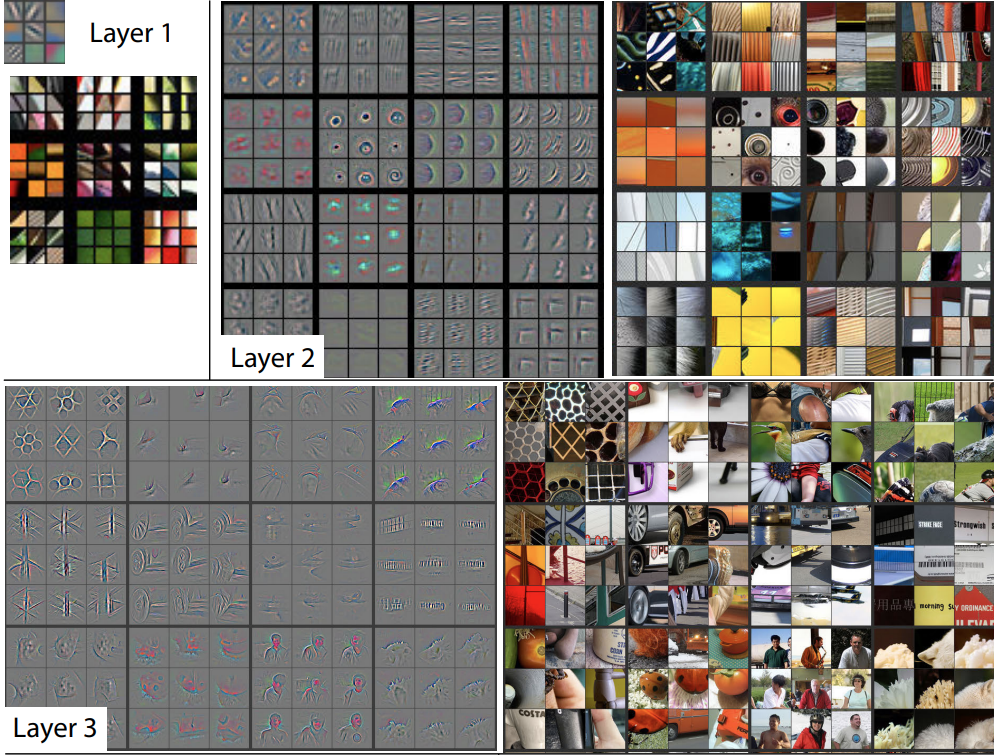
\includegraphics[width=1.0\textwidth]{images/zeiler_fergus_features.png}
    \caption{Hierarchical feature representations learned by a CNN.
        Layer 1 responds to oriented edges and simple colour gradients;
        Layer 2 captures corners, circular patterns and basic textures;
        Layer 3 represents more complex textures and object parts.
        Adapted from Zeiler and Fergus \cite{zeiler2014visualizing}.}
    \label{fig:cnn_features}
\end{figure}

Figure~\ref{fig:cnn_arch} shows the AlexNet architecture. The diagram is relevant here because it
illustrates the repeated pattern of convolution, pooling and fully connected layers that made deep
pixel-based recognition practical.

\begin{figure}[H]
    \centering
    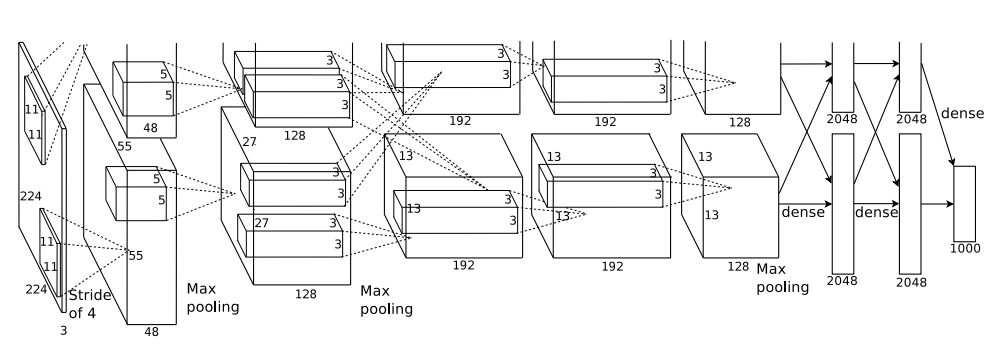
\includegraphics[width=0.9\textwidth]{images/alexnet_architecture.png}
    \caption{AlexNet architecture, showing stacked convolutional and pooling layers followed by fully connected layers. Source: Krizhevsky et al. \cite{krizhevsky2012imagenet}.}
    \label{fig:cnn_arch}
\end{figure}

In SLR context, pixel-based CNNs can learn discriminative visual patterns directly from raw video
frames. However, their main limitation is that they also receive information that may not define
the sign, including background, skin tone and recording conditions. When the available dataset is
limited, this can encourage the model to fit appearance correlations instead of sign structure.

\subsection{Pose Estimation Techniques}

Pose estimation involves predicting the spatial coordinates of anatomical points (landmarks) within
an image or video frame, which constitutes a regression task because it requires calculating
continuous numerical values rather than selecting a distinct class from a fixed set. In hand pose
estimation, many landmarks correspond to joints, which are anatomical articulations such as
knuckles, while fingertip landmarks mark the end of each finger. A regression-based pose estimator
therefore predicts landmark coordinates rather than a discrete class label.

Figure~\ref{fig:mediapipe_landmark_example} shows an example of the type of hand skeleton produced
by a landmark-based hand tracking system. The image illustrates how the visual hand region is
converted into a set of keypoints connected according to the anatomical structure of the hand.

\begin{figure}[H]
    \centering
    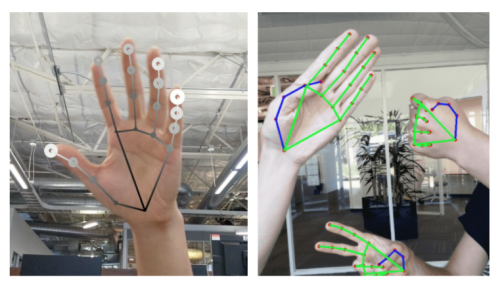
\includegraphics[width=0.65\textwidth]{images/landmark_image_paper.png}
    \caption{Rendered hand tracking result with hand landmarks and multi-hand tracking output. Source: Zhang et al. \cite{zhang2020mediapipehands}.}
    \label{fig:mediapipe_landmark_example}
\end{figure}

Pose pipelines are commonly organised as top-down or bottom-up systems. A top-down pipeline first
detects the relevant object or body part, then estimates landmarks inside the detected region. A
bottom-up pipeline first predicts candidate landmarks across the image, then groups them into
instances. Both approaches convert raw image evidence into a structured geometric representation.

MediaPipe Hands \cite{zhang2020mediapipehands} is a widely used hand pose estimation system. It
uses the top-down structure shown in Figure~\ref{fig:mediapipe_pipeline}: a hand detector proposes
a region of interest, and a landmark model estimates hand coordinates inside that cropped region.

\begin{figure}[H]
    \centering
    \begin{tikzpicture}[
            scale=0.78,
            every node/.style={font=\small},
            stage/.style={draw=black,rectangle,minimum width=2.10cm,minimum height=0.85cm,align=center,line width=0.45pt},
            input stage/.style={stage,fill=black!5},
            process stage/.style={stage,fill=black!12},
            output stage/.style={stage,fill=black!20,minimum width=2.45cm},
            flow/.style={->,black!70,line width=0.55pt},
            tracking/.style={->,black,line width=0.6pt}
        ]
        \node[input stage] (input) at (0,0) {Input\\frame};
        \node[process stage] (palm) at (3.00,0) {Palm\\Detection};
        \node[process stage] (crop) at (6.00,0) {Image\\Cropping};
        \node[process stage] (regress) at (9.00,0) {Landmark\\Regression};
        \node[output stage] (output) at (12.20,0) {21 hand\\landmarks output};

        \draw[flow] ([yshift=0.22cm]input.north east) --
        node[above,font=\scriptsize\itshape,fill=white,inner sep=1pt] {full image}
        ([yshift=0.22cm]palm.north west);
        \draw[flow] ([yshift=0.22cm]palm.north east) --
        node[above,font=\scriptsize\itshape,fill=white,inner sep=1pt] {bounding box}
        ([yshift=0.22cm]crop.north west);
        \draw[flow] ([yshift=0.22cm]crop.north east) --
        node[above,font=\scriptsize\itshape,fill=white,inner sep=1pt] {cropped hand}
        ([yshift=0.22cm]regress.north west);
        \draw[flow] ([yshift=0.22cm]regress.north east) --
        node[above,font=\scriptsize\itshape,fill=white,inner sep=1pt] {21 landmarks}
        ([yshift=0.22cm]output.north west);

        \draw[tracking]
        (regress.south) -- (9.00,-1.15) --
        node[below,font=\scriptsize\itshape,fill=white,inner sep=1pt] {Temporal tracking (next frame)}
        (6.00,-1.15) -- (crop.south);
    \end{tikzpicture}
    \caption{MediaPipe Hands pipeline. The palm detector locates the hand region on the first frame or when tracking is lost; the landmark model then regresses 21 three-dimensional landmarks inside the cropped region. Subsequent frames reuse the landmarks from the previous frame, avoiding running palm detection on every frame. Source: self-created, adapted from Zhang et al. \cite{zhang2020mediapipehands}.}
    \label{fig:mediapipe_pipeline}
\end{figure}

The process consists of the following stages:
\begin{enumerate}
    \item \textbf{Palm detection:} The full image frame is processed by a single-shot detector, which
          estimates a bounding region around the palm and defines the hand region of interest.
    \item \textbf{Image cropping:} The detected region is cropped and aligned around the hand,
          producing a normalised hand image for the landmark model.
    \item \textbf{Landmark regression:} The landmark model receives the cropped hand image and
          regresses the coordinates of 21 three-dimensional hand landmarks.
    \item \textbf{Temporal tracking:} When the hand remains visible, the pipeline reuses landmarks and
          region-of-interest information from the previous frame to obtain a continuous landmark
          sequence.
\end{enumerate}

For SLR, landmark sequences provide a compact description of hand shape and movement. They remove
much of the raw appearance signal and make it possible to derive additional geometric features such
as bone vectors, joint angles and distances between fingers. The cost of this abstraction is that
pose estimators may fail under occlusion, motion blur or unusual camera angles, and hand-only
landmarks omit non-manual cues such as facial expression and upper-body movement.

\section{Sequence Processing Architectures}
\label{sec:sequence_processing_architectures}

Isolated sign recognition is a temporal classification problem. This means that the input is not a
single image but an ordered sequence of feature vectors, one per frame or sampled time step. A
sequence processing layer therefore receives $\{\mathbf{x}_1,\mathbf{x}_2,\ldots,\mathbf{x}_T\}$
and produces a representation that accounts for temporal order.

\subsection{Recurrent Layers}

Recurrent Neural Networks (RNNs) process a sequence by maintaining a hidden state. At time $t$, the
layer combines the current input $\mathbf{x}_t$ with the previous hidden state $\mathbf{h}_{t-1}$:
\begin{equation}
    \mathbf{h}_t =
    \phi(\mathbf{W}_{xh}\mathbf{x}_t + \mathbf{W}_{hh}\mathbf{h}_{t-1} + \mathbf{b}_h)
\end{equation}
where $\phi$ is an activation function. The same parameters are shared at every time step, as shown
in Figure~\ref{fig:rnn_unrolled}. This sharing lets the layer process sequences of different
lengths while applying the same transition rule throughout the video.

\begin{figure}[H]
    \centering
    \begin{tikzpicture}[scale=0.95, every node/.style={font=\small}]
        \node[draw,minimum width=1.4cm,minimum height=0.8cm] (r1) at (0,0) {RNN};
        \node[draw,minimum width=1.4cm,minimum height=0.8cm] (r2) at (2.5,0) {RNN};
        \node[draw,minimum width=1.4cm,minimum height=0.8cm] (r3) at (5,0) {RNN};
        \node (x1) at (0,-1.2) {$\mathbf{x}_{t-1}$};
        \node (x2) at (2.5,-1.2) {$\mathbf{x}_{t}$};
        \node (x3) at (5,-1.2) {$\mathbf{x}_{t+1}$};
        \node (y1) at (0,1.2) {$\mathbf{h}_{t-1}$};
        \node (y2) at (2.5,1.2) {$\mathbf{h}_{t}$};
        \node (y3) at (5,1.2) {$\mathbf{h}_{t+1}$};
        \draw[->] (x1) -- (r1);
        \draw[->] (x2) -- (r2);
        \draw[->] (x3) -- (r3);
        \draw[->] (r1) -- (y1);
        \draw[->] (r2) -- (y2);
        \draw[->] (r3) -- (y3);
        \draw[->] (r1) -- (r2);
        \draw[->] (r2) -- (r3);
    \end{tikzpicture}
    \caption{Unrolled recurrent layer. The same recurrent computation is applied at each time step while the hidden state carries information forward. Source: self-created.}
    \label{fig:rnn_unrolled}
\end{figure}

Training recurrent layers uses Backpropagation Through Time (BPTT) \cite{werbos1990bptt}, which
unfolds the recurrent computation across the sequence and propagates the loss backwards through the
unfolded graph. As the number of time steps increases, standard recurrent layers frequently
encounter the vanishing gradient problem \cite{bengio1994longterm}. The gradient signal becomes too
small to preserve information from early time steps, which limits long-range temporal modelling.

The recurrent layer described above represents the baseline architecture. To address its
operational limitations, more sophisticated gated variants have been developed:
\begin{itemize}
    \item Long Short-Term Memory (LSTM) layers, which introduce a cell state and gates to regulate
          information flow.
    \item Gated Recurrent Unit (GRU) layers, which simplify the LSTM design while retaining gated
          memory.
\end{itemize}

\subsection{Long Short-Term Memory Layers}

Long Short-Term Memory (LSTM) layers were proposed by Hochreiter and Schmidhuber
\cite{hochreiter1997lstm} to improve the modelling of long temporal dependencies. An LSTM layer
maintains two vectors: the hidden state $\mathbf{h}_t$, which is exposed to the next layer or
output, and the cell state $\mathbf{C}_t$, which carries memory along the sequence.

The LSTM cell regulates this memory through gates. The forget gate controls which information is
removed from the cell state, the input gate controls which new information is written and the
output gate controls which part of the cell state becomes the hidden state.
Figure~\ref{fig:rnn_comparison} (a) represents these gates as $f$, $i$ and $o$, and shows how the
cell state $C$ provides a direct path for information flow.

This gated memory path is the mechanism referred to as the Constant Error Carousel. It reduces the
decay of the error signal during BPTT and allows the layer to retain information over longer time
spans than a simple recurrent layer. The cost is computational: each time step requires several
linear transformations, increasing both parameter count and training time.

\subsection{Gated Recurrent Unit Layers}

Gated Recurrent Unit (GRU) layers were introduced by Chung et al. \cite{chung2014gru} as a simpler
gated recurrent alternative. A GRU layer removes the separate cell state and stores memory directly
in the hidden state $\mathbf{h}_t$. It uses two gates, shown in Figure~\ref{fig:rnn_comparison}(b):
the update gate $z$ and the reset gate $r$.

\begin{figure}[H]
    \centering
    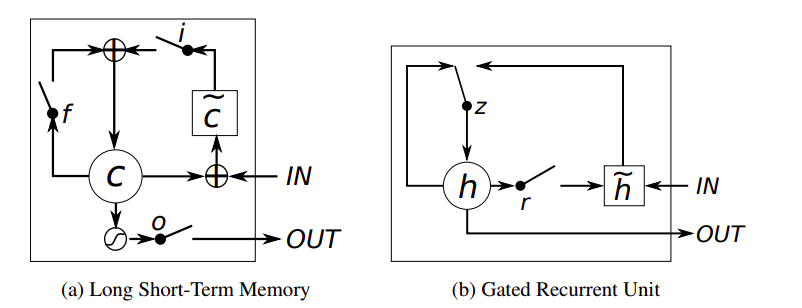
\includegraphics[width=0.8\textwidth]{images/gru_paper_diagram.png}
    \caption{Comparison of gated recurrent units. (a) LSTM cell with input, forget and output gates. (b) GRU cell with update and reset gates. Source: Chung et al. \cite{chung2014gru}.}
    \label{fig:rnn_comparison}
\end{figure}

The GRU gate equations at time $t$ are:
\begin{align}
    \mathbf{z}_t & = \sigma(\mathbf{W}_z\mathbf{x}_t + \mathbf{U}_z\mathbf{h}_{t-1} + \mathbf{b}_z) \\
    \mathbf{r}_t & = \sigma(\mathbf{W}_r\mathbf{x}_t + \mathbf{U}_r\mathbf{h}_{t-1} + \mathbf{b}_r)
\end{align}
The reset gate controls how much previous information is used to compute the candidate hidden state
$\tilde{\mathbf{h}}_t$. The update gate controls the interpolation between the previous hidden
state and the candidate state:
\begin{equation}
    \mathbf{h}_t = (1-\mathbf{z}_t)\odot\mathbf{h}_{t-1} + \mathbf{z}_t\odot\tilde{\mathbf{h}}_t
\end{equation}
When $\mathbf{z}_t$ is close to zero, the layer copies most of the previous hidden state. When it is
close to one, the layer replaces it with new information. This gives GRU layers a compact mechanism
for modelling temporal dependencies with fewer parameters than LSTM layers.

\section{Attention Mechanisms}
\label{sec:attention_mechanisms}

Attention mechanisms assign different weights to different parts of an input sequence. In neural
machine translation, Bahdanau et al. \cite{bahdanau2014neural} introduced attention to avoid
compressing a full source sentence into a single fixed-length vector. The same idea applies to
video recognition: not every frame contributes equally to the final prediction.

Given encoder states $\{\mathbf{h}_t\}_{t=1}^T$, an attention module computes a score $e_t$ for
each time step and normalises the scores with a softmax function:
\begin{equation}
    \alpha_t = \frac{\exp(e_t)}{\sum_{k=1}^{T}\exp(e_k)}, \quad e_t = a(\mathbf{s}, \mathbf{h}_t)
\end{equation}
where $a(\cdot)$ is a scoring function and $\alpha_t$ is the attention weight assigned to time step
$t$. The context vector is then computed as:
\begin{equation}
    \mathbf{c} = \sum_{t=1}^{T}\alpha_t\mathbf{h}_t
\end{equation}
Figure~\ref{fig:attention_mech} shows this weighted combination: the decoder state attends to
encoder annotations through weights $\alpha_{t,1},\alpha_{t,2},\ldots,\alpha_{t,T}$.

\begin{figure}[H]
    \centering
    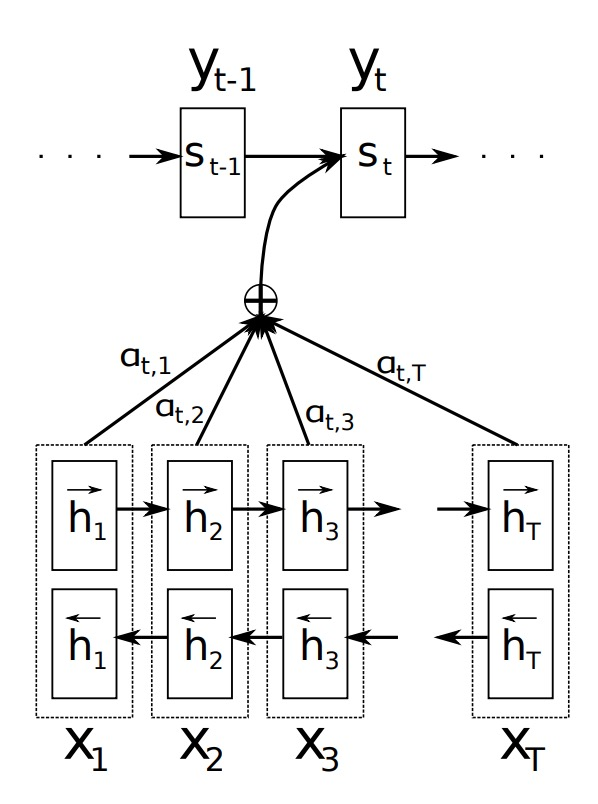
\includegraphics[width=0.5\textwidth]{images/temporal_attention.png}
    \caption{Attention mechanism in an encoder-decoder architecture. The context vector is a weighted sum of encoder annotations. Source: Bahdanau et al. \cite{bahdanau2014neural}.}
    \label{fig:attention_mech}
\end{figure}

For example, in an SLR clip of the sign \textit{drink}, the first frames may show the hand moving
towards the mouth, the central frames may contain the class-defining motion and the final frames
may show the hand returning to rest. Temporal attention can assign higher weights to the central
frames and lower weights to the preparation and recovery frames. This does not remove the need for
a sequence model; it adds a learned weighting stage over the temporal representation produced by
that model.

\subsection{Transformer Layers}

Transformer layers extend the attention idea by making self-attention the main operation of the
sequence model \cite{vaswani2017attention}. Instead of updating a hidden state step by step, as in
a recurrent layer, self-attention compares every position in the sequence with every other
position. Each time step is projected into query, key and value vectors. The query-key similarities
determine which positions are most relevant to each other, and the value vectors are combined
according to those attention weights.

This formulation allows a Transformer to model relationships between distant frames without passing
information through all intermediate time steps. It also supports parallel computation across the
sequence, which is useful when large datasets and long inputs are available. However, because the
model does not process frames in their natural order by default, positional information must be
added so that the network can distinguish earlier frames from later ones.

In SLR, Transformer-based models are relevant because signs often contain dependencies between
non-adjacent moments of the motion. At the same time, they can be more data-demanding than
recurrent layers, especially in small word-level datasets. For this reason, Transformers are best
understood in this work as attention-based sequence models to compare against recurrent
alternatives, rather than as an automatic replacement for LSTM or GRU layers.

\section{Related Work in Sign Language Recognition}
\label{sec:related_slr_work}

SLR research can be organised according to the recognition setting and the type of visual
representation used by the model. Survey work distinguishes between isolated sign recognition,
continuous sign recognition and sign language translation \cite{koller2020signlanguage,
rastgoo2021signlanguage,bragg2019signlanguagerecognition}. Isolated recognition assigns a single
gloss to a trimmed clip, which is the scope of this project. Continuous recognition must segment
and classify signs from longer streams, while translation must produce spoken-language text and
account for grammar, context and non-manual markers.

\paragraph{Detection-based approaches:}
Earlier vision pipelines often treated hands as regions to be detected before classification.
Modern object detectors such as Faster Region-based Convolutional Neural Network (Faster R-CNN)
\cite{ren2015fasterrcnn}, Single Shot MultiBox Detector (SSD) \cite{liu2016ssd}, EfficientDet
\cite{tan2020efficientdet} and the You Only Look Once (YOLO) family
\cite{redmon2016yolo,redmon2018yolov3} frame this problem as locating objects and assigning class
scores in images. YOLO is especially relevant for real-time hand detection because it performs
detection in a single forward pass, and YOLOv8 is a current implementation frequently used in
practical detection pipelines \cite{jocher2023yolov8}.

\paragraph{Pixel-based deep learning approaches:}
With the adoption of DNNs, many SLR systems moved from handcrafted descriptors towards models that
learn visual features directly from video frames. Pixel-based CNNs extract frame-level appearance
patterns, while recurrent layers model their temporal evolution and attention modules weight the
most informative moments of the sequence. Transformer-based work such as Sign Language Transformers
\cite{camgoz2020signlanguagetransformers} and STMC-Transformer \cite{yin2020stmc} shows how
attention-based sequence models have been applied to continuous recognition and translation
settings.

\paragraph{Pose-based approaches:}
Pose-based methods replace raw frames with landmark sequences, reducing dimensionality and limiting
the influence of background appearance. Bohacek and Hruz \cite{bohacek2022spoter} proposed a
pose-based Transformer for word-level SLR, while Sign2Pose \cite{eunice2023sign2pose} combines pose
features and Transformer-based gloss prediction on WLASL. This project is situated in the
pose-based line: MediaPipe Hands provides hand landmarks, and the recognition model evaluates
recurrent and attention-based temporal processing.

\paragraph{Datasets and evaluation context:}
Word-level ASL recognition is strongly associated with WLASL and MS-ASL. Li et al.
\cite{li2020wlasl} introduced WLASL together with benchmark comparisons for word-level recognition
from video, while Joze and Koller \cite{joze2019msasl} introduced MS-ASL as a larger ASL benchmark.
Both works helped move isolated SLR evaluation away from small curated vocabularies and towards
larger, noisier video collections. Large-scale work such as BSL-1K \cite{albanie2020bsl1k} also
highlights that dataset scale, weak supervision and cross-dataset transfer remain central concerns
in sign recognition research.

\section{Dataset Limitations}
\label{sec:sota_datasets}

SLR systems depend strongly on the datasets available for training and evaluation. Unlike general
image recognition, sign language recognition still lacks abundant large-scale benchmarks across
languages, domains and signer populations. Dataset design therefore shapes what a recognition model
can learn: the vocabulary determines the classification space, recording conditions affect visual
variation and annotation practice defines the gloss labels used for evaluation.

The main limitations are fourfold. First, many sign datasets contain a limited number of examples
per class, which makes it difficult to train high-capacity temporal models without overfitting.
Second, class imbalance is common: frequent signs tend to have many more examples than rare signs,
so aggregate accuracy may hide poor behaviour on under-represented glosses. Third, clips collected
from online sources introduce uncontrolled variation in camera quality, viewpoint, signer
appearance, background, duration and execution style. Finally, dataset attrition can occur when
source videos are removed or made private, reducing reproducibility over time.

These limitations affect how experimental results should be interpreted. A model can perform well
on a constrained benchmark while still struggling to generalise to new signers, recording
conditions or larger vocabularies. Auxiliary resources such as static alphabet datasets or
hand-detection corpora are useful for engineering stages, but they should not be treated as
word-level SLR benchmarks because they do not evaluate temporal sign dynamics.
\chapter{Objectives}
\setcounter{section}{0}

\lipsum[1-2]

\section{Main objective}

\lipsum[1-3]

\section{Specific objectives}

\lipsum[1-5]

\section{Validation methods}

\lipsum[1-5]

\chapter{Methodology and Work Plan Overview}
\setcounter{section}{0}

This chapter describes how the project was actually carried out: which materials and resources were
used, which technical methods are applied where, what process governed the day-to-day decisions, in
what sequence the work was done, and which constraints shaped every choice. The substance of
\emph{what was built} is reserved for the Technical Development chapter
(Section~\ref{sec:system_design} and following), and the substance of \emph{what was discovered
experimentally} is reserved for the Experiments chapter (Section~\ref{sec:exp_methodology} and
following); this chapter explains the \emph{way of working} that connects them.

% =============================================================================
\section{Materials and Resources}
\label{sec:plan_materials}
% =============================================================================

The project required four classes of resources: hardware, software stack, datasets, and
supervision. Each class is described briefly below and cross-referenced to the chapters where the
technical detail lives.

\paragraph{Hardware.} All training, evaluation, and landmark extraction were performed on a single local workstation
whose specification is the operational environment of Section~\ref{sec:operational_environment};
the full table of components and version constraints is Table~\ref{tab:operational_environment} and
is not repeated here. The relevant element for the work-plan discussion is the GPU: an NVIDIA
RTX~3050~Ti Laptop with 4\,GB of VRAM. The decision to keep the entire training pipeline on a local
GPU rather than on a cloud platform such as Google Colab or AWS was deliberate. Local execution
gives bit-for-bit reproducibility between consecutive runs, costs nothing per run (which mattered
because the iterative methodology described in Section~\ref{sec:plan_methodology} relaunches
experiments often), and removes the network-dependent latency that would otherwise penalise short
interactive runs. The 4\,GB VRAM ceiling is, in turn, the dominant hardware constraint discussed in
Section~\ref{sec:plan_constraints}.

\paragraph{Software stack.} The training and evaluation pipeline runs on Python~3.10 with PyTorch~2.x and CUDA~12.x. Pose
estimation uses MediaPipe Hands~0.10+, video decoding uses OpenCV~4.8+, and version control is
provided by Git with GitHub as remote host. The mobile client is built with React Native and Expo;
the inference server uses FastAPI~0.111 with Uvicorn~0.29. Documentation is authored in \LaTeX. The
exact version constraints are locked in \texttt{pyproject.toml} for the training package and in
\texttt{04\_server/requirements.txt} for the inference server, so that the operational environment
is reproducible from a clean clone of the repository (cross-reference:
Section~\ref{sec:operational_environment} and the reproduction guide at
\texttt{docs/reproducibility\_guide.md}).

\paragraph{Datasets.} Six datasets are used across the project: EgoHands and the Kaggle Hand Dataset for hand
localisation, Sign Language MNIST and the ASL Alphabet for letter classification, and WLASL and
MS-ASL for word recognition. Each dataset is formally defined in Section~\ref{sec:datasets}, where
attribute schema, licence considerations, and the role of each dataset in the experimental pipeline
are described. They are listed here only to make the resource inventory complete; the work-plan
discussion treats the datasets as external inputs whose acquisition, audit, and preparation costs
are accounted for in the corresponding phases of Section~\ref{sec:plan_workplan}.

\paragraph{Supervision and consultation resources.} The project was supervised by Mois\'es Mart\'inez Mu\~n\'oz through scheduled tutor meetings held
weekly or biweekly depending on the phase of the work. The most consequential technical decisions
of the project such as the pivot from pixel-based letter recognition to landmark-based word
recognition, the adoption of stratified $K$-fold cross-validation in place of test-time
augmentation, the cross-dataset extension to MS-ASL50 in addition to WLASL, and the introduction of
the multi-seed protocol, did not originate as solo decisions but as outcomes of these meetings. The
archived meeting notes preserve the directives that triggered each shift, and an internal audit
document was used to trace the meeting references cited in this chapter. Consultation resources
beyond the tutor consist of the literature reviewed in chapter~\ref{ch:sota} (notably the WLASL
benchmark, MediaPipe Hands, and the Bahdanau attention formulation) and a small number of
open-source repositories used as reference implementations: the WLASL benchmark distribution and
the MediaPipe Hands toolkit.

% =============================================================================
\section{Methods}
\label{sec:plan_methods}
% =============================================================================

This section is a compact catalogue of the technical methods the project relies on, presented
without re-justification. The theoretical background of each method is the subject of
chapter~\ref{ch:sota}, and the empirical evidence for each one is the subject of the Experiments
chapter (Section~\ref{sec:exp_methodology} and following); the role of this section is to make the
inventory explicit so that the rest of the chapter can refer to it.

The perception frontend uses MediaPipe Hands, a top-down two-stage pipeline that first detects the
palm and then regresses 21 three-dimensional keypoints per detected hand. The choice to operate on
landmarks instead of raw pixels is the central methodological decision of the project and is
justified in detail in Section~\ref{sec:exp_phase1}; the relevant point here is that all downstream
methods consume a landmark vector of 63 features per frame.

The temporal model is a bidirectional Gated Recurrent Unit with 256 hidden units per direction and
two stacked layers, followed by a Temporal Attention head implemented as an additive
(Bahdanau-style) softmax over the per-frame BiGRU outputs. A linear classifier projects the
attention-weighted context vector to the gloss vocabulary. This architecture is referred to
throughout the document as the GRU+Attention model and totals approximately 2.26\,million
parameters at the configurations reported in Section~\ref{sec:exp_methodology}. Two alternative
architectures appear in the comparison tables of Section~\ref{sec:exp_phase2}: a plain
bidirectional GRU baseline and a Transformer encoder with four layers and eight heads. They share
the input pipeline and the loss function with the champion model and differ only in the
sequence-modelling block.

Optimisation is performed with AdamW at learning rate $1\times10^{-3}$, weight decay
$5\times10^{-4}$, and label smoothing $0.1$ on the cross-entropy loss. The learning-rate schedule
is CosineAnnealingLR. Early stopping monitors the validation Top-1 accuracy with patience 30 epochs
and a maximum run length of 150 epochs. Skeletal augmentation during training combines rotation,
scaling, translation, additive Gaussian noise, and horizontal flip, applied per clip on the
landmark coordinates rather than on pixels.

Evaluation uses two complementary protocols. Stratified 5-Fold cross-validation runs on the WLASL30
vocabulary, with the dataset rebuilt by filtering WLASL100 down to the same 30 classes (332
samples) and the folds drawn so that the per-class distribution is preserved. The multi-seed
protocol runs the same configuration with three random seeds (42, 123, 2026) and reports the Top-1,
Top-5, Macro-F1, and Balanced Accuracy metrics as mean$\,\pm\,$standard deviation. Test-time
augmentation was deliberately excluded from the protocol after supervisory review identified it as
a source of biased inflation; the rationale is recorded in Section~\ref{sec:exp_methodology}.

Reproducibility is a method as much as a property. Every training and evaluation run produces an
\texttt{experiment\_manifest.json} that captures the git commit, the resolved configuration, the
hardware identifier, the wall-clock time, and the final metrics. Hyperparameters and dataset paths
live in YAML files under \texttt{configs/}, never in code, with a base configuration defining the
defaults shared across experiments and per-experiment files overriding only the fields they need.
The full reproduction procedure is documented in \texttt{docs/reproducibility\_guide.md}.

The exploratory phase of the project relied on two methods that no longer carry results in the
Experiments chapter but are listed here for completeness. The first is YOLOv8n hand detection, used
during Phase~B (see Section~\ref{sec:plan_workplan}) to localise hands from raw RGB frames. The
second is CNN-based pixel classification of static ASL letters. Both methods reached working
accuracy on their respective tasks and both were deprecated when the project pivoted to
landmark-based word recognition; Section~\ref{sec:exp_phase1} explains why.

% =============================================================================
\section{Methodology}
\label{sec:plan_methodology}
% =============================================================================

The project follows an iterative, experiment-driven methodology rather than a fixed waterfall plan,
because the technical direction shifted substantially after the early exploratory phase and any
plan that did not allow for that shift would have been discarded in February. The methodology is
not borrowed from CRISP-DM, Scrum, or any other process-software framework: those frameworks were
considered, but the development log documents a different and simpler pattern, applied repeatedly
across the lifetime of the project. That pattern is the basis of the methodology described here.

Each meaningful step of the project is organised as a four-stage loop. The loop starts with a
\emph{hypothesis} that is verifiable in principle: for example, ``landmark-based representation
outperforms pixel-based representation on WLASL30 within the available data budget,'' or ``a
sequence length of 64 frames produces lower seed-to-seed variance than 32 or 96.'' The loop
continues with \emph{implementation}: the relevant code changes are made in the \texttt{src/slr/}
package, augmented with whichever new YAML configuration the experiment requires, and committed to
git so that the run is anchored to a specific repository state. The loop then runs the
\emph{experiment}: the training script is launched, the manifest is written, and the metrics are
persisted alongside the model checkpoints in the experiment artifact directory. Finally, the loop
closes with \emph{reflection}: a devlog entry records what was attempted, what the result was,
whether the hypothesis was confirmed, and what the next step should be. If the hypothesis fails,
the next iteration starts from a new hypothesis informed by the failure rather than from the
original plan.

The pivot recorded in Section~\ref{sec:exp_phase1} is the most consequential application of this
loop. The project began with a pixel-based pipeline that targeted hand detection with YOLOv8n
followed by per-frame letter classification. Hand detection reached approximately 98\,\% mAP@0.5 on
the joint EgoHands+Kaggle test split and was, by any reasonable measure, working. Letter
classification was equally tractable on the static-frame benchmarks. The combined pipeline,
however, surfaced a structural observation that no incremental tuning would have removed: the
bottleneck of the system was not localising the hand but representing the dynamic content of the
sign. The four-stage loop responded to that observation by retiring the pixel-based recognition
stage and replacing it with the landmark-based word-recognition pipeline that is the subject of
every subsequent chapter. The pivot was a methodological consequence, not an arbitrary scope
change: the iterative loop is what made the pivot possible, and the development log makes the
rationale auditable in retrospect.

Two further properties of the methodology are worth making explicit because they show up repeatedly
in the Technical Development and Experiments chapters that follow. The first is the role of tutor
meetings as control points. The most impactful technical decisions of the project were made jointly
with the supervisor at scheduled meetings rather than unilaterally between iterations. These
decisions included removing test-time augmentation from the evaluation protocol after supervisory
review, restructuring the State of the Art chapter as a hierarchical
CNN$\rightarrow$RNN$\rightarrow$LSTM$\rightarrow$GRU theory progression, adopting Google's AI
Principles during the ethics review phase, and splitting the experimental work into quantitative
and qualitative tracks during the final experimental review. The meetings act as low-frequency
external feedback that the four-stage loop, on its own, would not provide.

The second property is the introduction of the multi-seed protocol described in
Section~\ref{sec:plan_methods}. The protocol is a direct response to a tutor concern about
reproducibility raised in early April~2026: a single-seed Top-1 figure on the 34-sample WLASL30
test split is bounded below in resolution by the granularity of one misclassification
($\approx$2.94\,pp), and a single number at that resolution is indistinguishable from
initialisation noise. The methodology absorbed the concern by adding a new ``aggregate over three
seeds'' step to every headline experiment going forward and by retroactively applying it to the
sequence-length sweep and to MS-ASL50. This is a concrete example of the iterative methodology
incorporating supervision: the protocol that distinguishes a defensible thesis number from a noisy
point was added in response to a single conversation, propagated through the codebase by adding a
small number of YAML files, and reflected in Section~\ref{sec:exp_methodology} as the statistical
backbone of the experimental claims.

Documentation is treated as a continuous side effect of the loop rather than as a separate phase.
The development log contains one entry per meaningful session, dated, scoped to a specific session
name, and indexed centrally. The log is the primary source from which the work plan in
Section~\ref{sec:plan_workplan} is reconstructed; without it, the chronology of the project would
be unrecoverable from the code alone.

% =============================================================================
\section{Work Plan}
\label{sec:plan_workplan}
% =============================================================================

The executed work plan was reconstructed from the original proposal, recorded development notes,
experiment artifacts, and supervision notes. The plan is organised into seven phases (A--G). The
first two phases correspond closely to the proposal-era plan, while the remaining phases reflect
the methodological pivot from static, pixel-based recognition to landmark-based word-level ASL
recognition.

\paragraph{Phase A: Project framing and proposal.} The project formally started in the first week of January~2026 with problem definition, preliminary
literature review, scope selection, and proposal preparation. This phase defined the accessibility
motivation, the initial system architecture, the first work schedule, and the research direction.
No model training was carried out at this stage; the main output was the approved project proposal
and its initial planning material.

\paragraph{Phase B: Hand detection and static letter recognition.} The initial technical work explored the proposal's first recognition route: localising hands in
images and classifying static ASL letters. A YOLOv8n detector was trained on a combined EgoHands
and Kaggle Hand Dataset corpus, and CNN-based classifiers were explored on static ASL alphabet
datasets. These components reached working performance on their own tasks, but they also revealed a
limitation in the original direction: the central research challenge was not hand localisation, but
representing the temporal structure of complete signs.

\paragraph{Phase C: Landmark pivot and WLASL30 baseline.} In late January and February 2026, the project pivoted from pixel-based letter recognition to
word-level recognition using MediaPipe hand landmarks. WLASL30 was built as the first controlled
benchmark, and several sequence models were compared under the same landmark input representation.
The GRU+Attention architecture emerged as the strongest baseline because it combined a recurrent
temporal model with an attention mechanism able to focus on the most informative frames. After
supervisory review, test-time augmentation was excluded from the final evaluation protocol, and the
WLASL30 result was strengthened through stratified $K$-fold validation.

\paragraph{Phase D: Vocabulary scaling and ethical framework.} Once the GRU+Attention model had been selected, the next phase tested how the approach behaved as
the WLASL vocabulary increased beyond the initial 30-class setting. The model was retrained on
progressively larger WLASL subsets to quantify the effect of vocabulary size and per-class data
scarcity. In parallel, the ethical and social-impact chapter was developed, including the
accessibility motivation, privacy implications of landmark-based representations, bias
considerations, reproducibility, and the responsible-deployment limits of the prototype.

\paragraph{Phase E: Runtime prototype.} In April 2026, the technical work expanded from offline training to a runtime proof of concept. A
mobile client and FastAPI server were integrated so that short clips could be captured, sent for
inference, and returned as Top-$K$ word predictions. Additional prototype features included
text-to-speech, model selection from the client, and a heuristic continuous-prediction demo mode
based on overlapping windows. This phase demonstrates end-to-end feasibility, but it is not treated
as the main research result; the quantitative contribution remains the landmark-based recognition
pipeline and its validation.

\paragraph{Phase F: Refactoring and cross-dataset validation.} The notebook-based experimental code was consolidated into a modular Python package, with
configuration-driven training, structured experiment manifests, reusable evaluation scripts, and
preserved checkpoints and plots. This refactor improved reproducibility and made it possible to
rerun the same pipeline across datasets. MS-ASL50 was then added as an independent validation
benchmark, and the final evaluation protocol incorporated multi-seed runs, a sequence-length sweep,
cross-dataset validation, and comparison against the WLASL results.

\paragraph{Phase G: Documentation and qualitative validation design.} The final phase focused on thesis writing, result consolidation, figure and table preparation, and
the design of a qualitative validation protocol for the runtime prototype. The experimental chapter
was organised into quantitative and qualitative tracks: the quantitative track reports completed
model evaluations, while the qualitative track defines the participant protocol and analysis plan
for future usability evidence. This phase remains open at the time of this intermediate submission
and will be completed with the final thesis revision and qualitative data integration.

Figure~\ref{fig:work_plan_timeline} summarises the executed work plan. The chart follows the seven
phases described above and highlights the main deviation from the initial proposal: the pivot from
static letter recognition to landmark-based word-level recognition.

\image{plan/work_plan_gantt.png}{0.95}{Project Gantt chart showing the executed work plan grouped into seven phases, from project framing and initial hand-detection experiments to landmark-based word recognition, cross-dataset validation, prototype integration, and final documentation. Source: self-created with GanttProject.}{fig:work_plan_timeline}

\FloatBarrier

% =============================================================================
\section{Constraints and Limitations}
\label{sec:plan_constraints}
% =============================================================================

This section catalogues the constraints that shaped the work plan and the methodology rather than
the experimental results. Limitations of the experimental conclusions themselves, including
standard deviations, test-set granularity, and single-architecture cross-dataset validation, are
treated separately in Section~\ref{sec:exp_limitations}.

The first constraint is time. The project was developed in parallel with a software-engineering
internship, which restricted the number of contiguous hours that could be dedicated to it in any
given week. The iterative methodology described in Section~\ref{sec:plan_methodology} is in part a
response to this constraint: a four-stage loop with an explicit devlog entry per session is what
makes it possible to resume the project after a multi-day pause without losing the local context.
Without the log, the cost of re-entering a problem after an interruption would have dominated the
cost of solving it.

The second constraint is hardware. Every training and evaluation run executed on a single NVIDIA
RTX~3050~Ti Laptop with 4\,GB of VRAM. This ceiling propagated into multiple design choices:
\texttt{max\_frames}\,=\,64 was selected partly because longer sequences exceeded the memory budget
at batch size 32, the GRU+Attention model was sized at approximately 2.26\,million parameters
rather than the parameter counts typical of large Transformers, and the Transformer baseline that
does appear in Section~\ref{sec:exp_phase2} uses a relatively narrow $d_{\mathrm{model}}=256$ for
the same reason. A cloud GPU was considered and rejected: per-run cost predictability and
bit-for-bit reproducibility between consecutive runs were judged more valuable than the additional
VRAM.

The third constraint is data availability. Both word-recognition datasets used in the project are
reconstructed from external sources rather than distributed directly, and both have lost a
measurable fraction of their original clips. WLASL relies on URLs that have decayed since the
dataset was published, and the MediaPipe detection rate on the surviving WLASL clips is
approximately 69\,\%, which limits the effective per-clip information content. MS-ASL is
reconstructed from per-instance YouTube URLs, and the reconstruction audit records a download
success rate of 65.9\,\% (16{,}816 of 25{,}513 clips). The MS-ASL50 subset, rather than the more
conventional MS-ASL30, is a direct response to this constraint: only six of the top-30 MS-ASL
classes meet the strict 30/5/5 train/val/test threshold from current YouTube state, so an MS-ASL30
reproduction would have been statistically indefensible (cf.\ Section~\ref{sec:exp_msasl}).

The fourth constraint is evaluator availability. Until the qualitative validation protocol
described in Section~\ref{sec:exp_qualitative} executes, the author is the only evaluator and the
only experimenter on the project. This is a standard configuration for an undergraduate
final-degree project and is acceptable for the quantitative work, where the evaluation is fully
automated and reproducible from a manifest. It does, however, mean that the cognitive bias of the
experimenter is uncontrolled at the design level. The qualitative protocol is structured so that
the analysis plan is fixed in advance of data collection, in the spirit of pre-registration,
precisely to mitigate this bias once the protocol runs.

The fifth constraint is linguistic scope. The project validates a single sign language, American
Sign Language, and uses ASL exclusively for both the WLASL and MS-ASL benchmarks. The pipeline
contains no ASL-specific assumptions, and every component that consumes landmarks could in
principle be retrained on a different sign language given a comparable benchmark. The validation
has not been done, however, and any claim about transfer to Spanish Sign Language, British Sign
Language, or any other variety is therefore future work.

The sixth and most general constraint is that the iterative, experiment-driven methodology
described in Section~\ref{sec:plan_methodology} is, by construction, incompatible with the literal
execution of the Gantt that the project proposal recorded in January~2026. The Gantt scheduled hand
localisation, static handshape recognition, dynamic sign recognition, temporal fusion and decoding,
language generation, mobile prototype, component integration, and validation tests as a sequence of
rigid intervals; the methodology actually applied retired the Static Handshape Recognition track in
favour of word-level recognition, replaced the proposed PaliGemma language-generation step with a
direct gloss-to-text mapping, and folded the Temporal Fusion stage into the GRU+Attention model.
This divergence is not a planning failure but a deliberate property of the methodology. The tutor
meeting notes document the moments at which each scope change was approved, and the devlog and
meeting notes together act as the audit trail that links the proposal-era plan to the executed
plan.

\chapter{Technical Development}
\setcounter{section}{0}

This chapter describes the research and engineering foundations of this FDP: how the recognition
solution is structured into independent stages, the methodological investigations that informed the
choice of algorithms and hyperparameters, and the functional capabilities provided by each stage.
It also details the execution environment and the requirements that drove the architectural design.
Finally, it describes the experimental datasets that feed the recognition pipeline.

\section{Solution design}
\label{sec:system_design}

The solution is structured as a modular three-stage architecture, integrating research-driven
methods across data preparation, model training and evaluation, and runtime inference. The stages
are physically separated (different processes and different machines in the execution environment)
but share a single source of truth for data formats and trained model artefacts, so a checkpoint
produced during model training can be served unchanged during runtime inference.
Figure~\ref{fig:system_overview} shows the solution architecture and its execution flow.

\clearpage
\begin{landscape}
    \thispagestyle{empty}
    \begin{figure}[H]
        \centering
        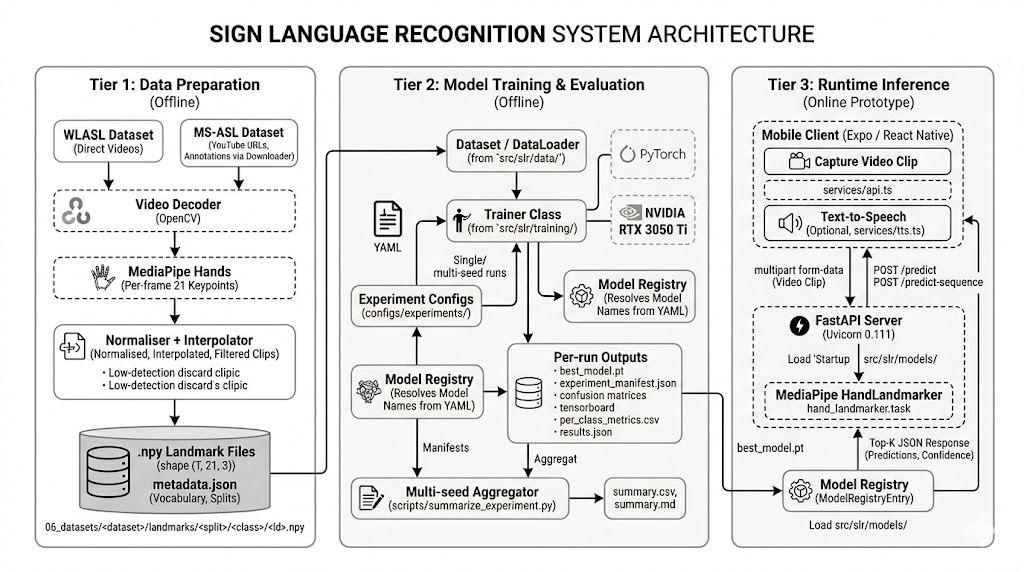
\includegraphics[width=\linewidth,height=1.0\textheight,keepaspectratio]{./images/architecture/system_overview.png}
        \caption{Solution architecture showing the data preparation, training and evaluation, and runtime inference stages. Source: self-created from the implemented pipeline.}
        \label{fig:system_overview}
    \end{figure}
\end{landscape}
\clearpage

\subsection{Stage 1: Data preparation}
\label{subsec:data_preparation}

The data preparation stage converts raw benchmark videos into landmark sequences that can be used
by the training and inference stages. It corresponds to the first two stages of the recognition
pipeline introduced in Section~\ref{subsec:recognition_pipeline}, namely video acquisition and
decoding, and landmark extraction and normalisation. This section decomposes those stages into five
execution phases:

\begin{enumerate}
    \item \textbf{Video acquisition.} The input is the official Word-Level American Sign Language
          (WLASL) distribution or the Microsoft American Sign Language (MS-ASL) annotation files.
          WLASL clips are downloaded from the dataset distribution, while MS-ASL clips are
          reconstructed from the referenced YouTube videos. The output is a local set of labelled
          video clips aligned with their gloss and split metadata.
    \item \textbf{Clip decoding and temporal trimming.} OpenCV decodes each video frame by frame.
          For MS-ASL, each source video is trimmed with the per-instance \texttt{(start\_time,
              end\_time)} pair. The output is an ordered frame sequence for one sign instance.
    \item \textbf{Hand landmark extraction.} MediaPipe Hands estimates 21 three-dimensional
          landmarks per valid frame. The output for each frame is a structured hand representation
          with coordinates for the wrist, finger joints and fingertips.
    \item \textbf{Geometric normalisation and missing-frame handling.} Each frame is wrist-centred
          and length-normalised by the wrist-to-middle-finger distance. Frames where MediaPipe fails
          to detect a hand are linearly interpolated from neighbouring valid frames, and clips whose
          detection rate falls below 0.3 are discarded.
    \item \textbf{Serialisation.} Each surviving clip is stored as a per-clip \texttt{.npy} array
          of shape $(T, 21, 3)$. The accompanying \texttt{metadata.json} records the dataset name,
          gloss vocabulary, split assignments and source-video identifiers.
\end{enumerate}

This stage is implemented in \texttt{src/slr/data/} and exposed through the
\texttt{scripts/extract\_landmarks\_*.py} entry points.

\subsection{Stage 2: Model training and evaluation}
\label{subsec:model_training_evaluation}

The training and evaluation stage turns landmark sequences into reproducible model comparisons. Its
execution follows four phases:

\begin{enumerate}
    \item \textbf{Configuration resolution.} The input is a YAML configuration under
          \texttt{configs/}. The file specifies the dataset path, model identifier, optimiser,
          sequence length and evaluation settings. Shared defaults are declared in
          \texttt{configs/base/gru\_attention.yaml}, and experiment-specific files override only
          the fields that change.
    \item \textbf{Model construction.} The registry in \texttt{src/slr/models/} resolves the model
          identifier into one of the implemented sequence architectures. The supported identifiers
          are \texttt{gru\_baseline}, \texttt{gru\_attention} and \texttt{transformer}.
    \item \textbf{Optimisation and evaluation.} The trainer in \texttt{training/trainer.py}
          optimises the selected architecture and evaluates it through the shared evaluator in
          \texttt{evaluation/}. The same trainer supports the multi-seed protocol used to report
          mean and standard deviation in the experiments chapter.
    \item \textbf{Artefact generation.} Each run produces a self-contained directory with the best
          checkpoint by validation Top-1, the training history, confusion matrices, per-class
          metrics and an \texttt{experiment\_manifest.json} recording git commit, hardware,
          runtime, hyperparameters and final metrics.
\end{enumerate}

The experiment-tracking code is implemented in \texttt{tracking/manifest.py} and
\texttt{tracking/git\_utils.py}.

\subsection{Stage 3: Runtime inference}
\label{subsec:runtime_inference}

The runtime inference stage integrates the trained recogniser into a mobile/server proof of
concept. Its execution follows five phases:

\begin{enumerate}
    \item \textbf{Video capture.} The React Native and Expo client in
          \texttt{03\_app/signtotext-expo/} records a short video clip with the device camera.
    \item \textbf{Request submission.} The client sends the clip to the FastAPI server in
          \texttt{04\_server/main.py} through the REST client implemented in
          \texttt{services/api.ts}.
    \item \textbf{Server-side preprocessing.} The server applies the same MediaPipe landmark
          extraction, normalisation and sequence preparation used in the data preparation stage.
    \item \textbf{Prediction.} The server loads the requested checkpoint from the model registry
          and returns Top-K predictions with confidence scores through \texttt{POST /predict}.
          The \texttt{POST /predict-sequence} endpoint provides a heuristic continuous-sequence
          variant.
    \item \textbf{Client response.} The client displays the prediction shortlist and can pass the
          Top-1 label to the text-to-speech service in \texttt{services/tts.ts}.
\end{enumerate}

The server reuses the \texttt{src/slr/} package directly, so the inference code path remains
aligned with the evaluation code path.

\subsection{Description of functional features}
\label{sec:functional_features}

The solution exposes six high-level capabilities. Each one is justified by the technical decision
it embodies, so this list doubles as a record of why the architecture took its current shape.

\begin{itemize}
    \item \textbf{F1: Landmark-based input pipeline.} Each frame is reduced from a $224 \times 224$ RGB tensor to 63 floating-point landmark coordinates, a roughly 2{,}389$\times$ dimensionality reduction. The choice removes background and skin-tone signal at source, which both shrinks the model and disconnects recognition accuracy from appearance bias.
    \item \textbf{F2: Multi-seed training protocol.} The trainer supports running the same configuration across multiple random seeds and aggregating the metrics with mean and standard deviation. Without this protocol, a single-seed Top-1 figure on a small test set is indistinguishable from noise; with it, a 2--3 percentage-point standard deviation can be reported alongside every headline number.
    \item \textbf{F3: Architecture-agnostic training loop.} The same \texttt{Trainer} accepts three model identifiers through a registry lookup: \texttt{gru\_baseline} is a bidirectional GRU architecture without attention, \texttt{gru\_attention} is the selected GRU architecture with a temporal attention layer, and \texttt{transformer} is a self-attention architecture used as a comparison baseline. This makes the architecture comparison reproducible: only the model field of the YAML changes between runs, every other variable stays fixed.
    \item \textbf{F4: Cross-dataset validation.} The same pipeline runs unmodified on WLASL and on MS-ASL. Only the dataset path and the gloss vocabulary differ between the two configurations; nothing in the model, optimiser or loss is dataset-specific, which is what makes the cross-dataset comparison fair.
    \item \textbf{F5: Reproducible experiment tracking.} Every run writes an \texttt{experiment\_manifest.json} that captures git commit, dataset metadata, hyperparameters, hardware, runtime, and final metrics in one place. A future user can reconstruct the exact configuration of any historical run from this single file.
    \item \textbf{F6: Top-K predictions in inference.} The runtime API returns Top-1 and Top-5 candidates with confidence scores instead of forcing a single answer. This matches the way the model itself is evaluated and lets the client surface a shortlist when the Top-1 confidence is low.
\end{itemize}

For example, the \texttt{experiment\_manifest.json} generated for the MS-ASL50 seed 2026 run
records the dataset identifier, random seed, split sizes, GRU+Attention configuration, hardware,
runtime, checkpoint path and final metrics, including 71.19\% Top-1 and 91.53\% Top-5 accuracy.
This is the concrete output produced by the reproducible experiment-tracking feature.

\subsection{Operational Environment}
\label{sec:operational_environment}

Training and landmark extraction were performed in the local development environment; the runtime
prototype was tested with a paired mobile client and an HTTP server.
Table~\ref{tab:operational_environment} summarises the hardware, software runtime and storage
formats under which the results in this FDP were produced.

\begin{table}[H]
    \centering
    \small
    \renewcommand{\arraystretch}{1.25}
    \caption{Operational environment for training, landmark extraction, and runtime inference.}
    \label{tab:operational_environment}
    \begin{tabular}{@{}p{4.2cm} p{9.0cm}@{}}
        \toprule
        \textbf{Environment area} & \textbf{Specification}                                                          \\
        \midrule
        Operating system          & Ubuntu 24.04 LTS (training and server); cross-platform (mobile client).         \\
        CPU                       & Multi-core x86\_64 (local laptop).                                              \\
        GPU                       & NVIDIA RTX 3050 Ti Laptop, 4\,GB VRAM, CUDA 12.x.                               \\
        Python                    & 3.10 (project); 3.11 supported via \texttt{requires-python = ">=3.10"}.         \\
        Deep learning framework   & PyTorch 2.x with CUDA support.                                                  \\
        Pose estimation           & MediaPipe Hands 0.10+ (\texttt{HandLandmarker}).                                \\
        Video processing          & OpenCV 4.8+.                                                                    \\
        Mobile client framework   & React Native + Expo.                                                            \\
        Backend                   & FastAPI 0.111 with Uvicorn 0.29.                                                \\
        Persistence               & JSON manifests, \texttt{.npy} landmark files, \texttt{.pt} PyTorch checkpoints. \\
        Version control           & Git.                                                                            \\
        \bottomrule
    \end{tabular}
\end{table}

The detailed installation and execution procedure is not repeated in this section. It belongs to
the user manual appendix, where the environment setup, dataset preparation, training commands,
evaluation commands and server execution procedure are described together.

\section{Requirements}
\label{sec:requirements}

\subsection{Description of requirement attributes}

For the textual description of the different identified requirements, a set of attributes has been
selected to describe each requirement. Below is a description of the meaning of each attribute
used:

\begin{itemize}
    \item \textbf{Code}: A unique abbreviated identifier for the requirement. It is constructed using the requirement type code followed by a hyphen and three digits. Requirements are divided into functional and non-functional requirements. The codes used are \textbf{FR} for Functional Requirements and \textbf{NFR} for Non-Functional Requirements. For example: \texttt{FR-001}.

    \item \textbf{Name}: Extended identification of the requirement.

    \item \textbf{Description}: A basic description of the identified requirement.

    \item \textbf{Source}: Indicates the source through which the requirement was identified. This value usually corresponds to one or more use case codes.

    \item \textbf{Necessity}: Determines the degree of implementation required for the requirement. The possible values are:
          \begin{itemize}
              \item \textbf{Essential}: The requirement must be implemented.
              \item \textbf{Desirable}: It is preferable to implement the requirement, but it is not mandatory.
              \item \textbf{Optional}: The requirement may be implemented, but it is neither important nor mandatory.
          \end{itemize}

    \item \textbf{Priority}: Defines the importance of the requirement, allowing the order in which requirements are included in the design and implementation process to be established. The possible values are:
          \begin{itemize}
              \item \textbf{High}: The requirement must be implemented in the early stages of development.
              \item \textbf{Medium}: The requirement should be implemented once high-priority requirements have been completed.
              \item \textbf{Low}: The requirement should be implemented in the final stages of development. These requirements do not affect the correct functioning of the system.
          \end{itemize}

    \item \textbf{Stability}: Defines the stability of the requirement throughout the software life cycle. This indicates whether the requirement may be modified during the life cycle. The possible values are:
          \begin{itemize}
              \item \textbf{Stable}: The requirement will not change during the system life cycle.
              \item \textbf{Unstable}: The requirement may change during the system life cycle.
          \end{itemize}

    \item \textbf{Verifiability}: Defines the degree to which a requirement can be verified, that is, the extent to which it is possible to confirm that the requirement has been implemented in the developed system. The possible values are:
          \begin{itemize}
              \item \textbf{High}: It is possible to verify that the requirement has been implemented. These requirements usually correspond to core system functionalities.
              \item \textbf{Medium}: It is possible to verify that the requirement has been implemented, but it requires complex testing or inspection of the source code.
              \item \textbf{Low}: It is difficult, or in some cases impossible, to verify whether the requirement has been implemented.
          \end{itemize}
\end{itemize}

\subsection{Functional Requirements}
\label{sec:functional_requirements}

The system specifies four functional requirements covering the core recognition pipeline (FR-001,
FR-002), the experiment-tracking infrastructure (FR-003), and statistical validation through
multi-seed training (FR-004).

\requirement{./tables/requirement_FR_001}{FR-001: Landmark extraction from video clips}{tab:requirement_FR_001}
\requirement{./tables/requirement_FR_002}{FR-002: Word-level sign classification}{tab:requirement_FR_002}
\requirement{./tables/requirement_FR_003}{FR-003: Reproducible experiment tracking}{tab:requirement_FR_003}
\requirement{./tables/requirement_FR_004}{FR-004: Multi-seed training support}{tab:requirement_FR_004}
\FloatBarrier

\subsection{Non-functional Requirements}
\label{sec:non_functional_requirements}

Three non-functional requirements characterise quality attributes of the system: runtime
performance (NFR-001), code quality and modularity (NFR-002), and documentation completeness
(NFR-003).

\requirement{./tables/requirement_NFR_001}{NFR-001: Inference latency}{tab:requirement_NFR_001}
\requirement{./tables/requirement_NFR_002}{NFR-002: Modular code architecture}{tab:requirement_NFR_002}
\requirement{./tables/requirement_NFR_003}{NFR-003: Documentation completeness}{tab:requirement_NFR_003}
\FloatBarrier

% =============================================================================
\section{Datasets}
\label{sec:datasets}
% =============================================================================

This FDP spans two recognition tasks with different data requirements: hand localisation from still
images and word-level sign language recognition from video. Six datasets are therefore used across
the experimental pipeline. This section formalises the properties of each dataset by first defining
a common set of descriptive attributes, then presenting a comparative table and finally describing
each dataset with the same structure: metadata and technical specifications, composition and
volume, source, and preparation.

% 3.X.1 Attribute Definitions
\subsection{Dataset Attribute Definitions}
\label{subsec:dataset_attributes}

To ensure a consistent and unambiguous characterisation of every dataset, the following attributes
are used in Table~\ref{tab:datasets_comparison}. Each attribute captures a distinct dimension
relevant to dataset selection, reproducibility, and the interpretation of experimental results:

\begin{itemize}

    \item \textbf{ID}: A unique alphanumeric identifier assigned to each dataset within this FDP. The prefix \texttt{DS-} followed by a two-digit index allows unambiguous cross-referencing in subsequent chapters when reporting experimental configurations and results.

    \item \textbf{Name}: The official or widely-used name of the dataset as it appears in the literature or on its hosting platform.

    \item \textbf{Year}: The year of original publication or first public release. This contextualises the dataset within the chronological development of the field and helps evaluate whether it reflects current data collection practice.

    \item \textbf{Task}: The specific sub-task for which the dataset was designed. Three task categories appear in this FDP:
          \begin{itemize}
              \item \textbf{Hand Detection}: the dataset provides annotated bounding boxes or segmentation masks marking the location of hands in images.
              \item \textbf{Letter Recognition}: the dataset provides labelled static images of individual American Sign Language (ASL) letter signs.
              \item \textbf{Word Recognition}: the dataset provides labelled video clips of complete ASL word signs, requiring temporal modelling.
          \end{itemize}

    \item \textbf{Samples}: The total number of annotated data instances. For image datasets, this equals the number of images; for video datasets, it equals the number of individual video clips. Where a subset of the full dataset was used in this FDP, this is noted in the individual descriptions.

    \item \textbf{Classes}: The number of distinct output categories. For hand detection datasets this is always 1 (the single \textit{hand} class); for sign language datasets it corresponds to vocabulary size, meaning the number of distinct letters or word glosses.

    \item \textbf{Format}: The storage format and annotation type of the raw data. This attribute specifies whether instances are static images or video clips, the image resolution where relevant, and the form of ground-truth annotation, such as bounding box coordinates in XML, pixel-level segmentation masks, image class labels or video-level class labels.

    \item \textbf{Input Representation}: Whether the models trained on this dataset consume \textit{pixel-based} data (raw RGB or greyscale image/video frames) or \textit{landmark-based} data (structured three-dimensional keypoint coordinates extracted by a pose estimator such as MediaPipe). Pixel-based inputs preserve full visual detail but are high-dimensional and sensitive to background, lighting and signer appearance. Landmark-based inputs are compact and less exposed to visual variability, at the cost of depending on a reliable keypoint extractor.

\end{itemize}

% 3.X.2 Comparative Overview
\subsection{Comparative Overview}
\label{subsec:dataset_overview}

Table~\ref{tab:datasets_comparison} provides a high-level comparison of the six datasets used in
this FDP. Datasets DS-01 and DS-02 support the hand localisation pipeline. Datasets DS-03 and DS-04
were used in the initial letter-level classification phase, which was later superseded by
word-level recognition. Datasets DS-05 and DS-06 are the video benchmarks used for the final
landmark-based ASL recognition pipeline.

\begin{table}[H]
    \centering
    \scriptsize
    \setlength{\tabcolsep}{3pt}
    \renewcommand{\arraystretch}{1.25}
    \caption{Comparative overview of all datasets used in this FDP.}
    \label{tab:datasets_comparison}
    \begin{tabular}{@{}p{0.8cm} p{2.7cm} p{0.7cm} p{2.0cm} p{1.45cm} p{1.3cm} p{2.25cm}@{}}
        \toprule
        \textbf{ID} & \textbf{Name}       & \textbf{Year} & \textbf{Task}  & \textbf{Samples} & \textbf{Classes} & \textbf{Format}            \\
        \midrule
        DS-01       & EgoHands            & 2015          & Hand Detection & 4,800            & 1                & Images + seg.\ masks       \\
        DS-02       & Kaggle Hand Dataset & 2023          & Hand Detection & $\sim$4,200      & 1                & Images + BBox (XML)        \\
        DS-03       & Sign Language MNIST & 2017          & Letter Recog.  & 34,627           & 24               & 28$\times$28 greyscale CSV \\
        DS-04       & ASL Alphabet        & 2018          & Letter Recog.  & 87,000           & 29               & 200$\times$200 RGB JPG     \\
        DS-05       & WLASL               & 2020          & Word Recog.    & 21,083           & 2,000            & RGB video clips            \\
        DS-06       & MS-ASL              & 2018          & Word Recog.    & 25,513           & 1,000            & RGB video clips, YouTube   \\
        \bottomrule
    \end{tabular}
\end{table}

% 3.X.3 Hand Detection Datasets
\subsection{Hand Detection Datasets}
\label{subsec:datasets_hd}

Datasets DS-01 and DS-02 are used jointly to train the hand localisation module based on You Only
Look Once version 8 nano (YOLOv8n). Combining the two sources increases viewpoint diversity: an
egocentric-only detector may fail when the camera is positioned at eye level, while a detector
trained only on third-person images may struggle with first-person perspectives. After merging,
duplicate removal and a stratified train/validation/test split, the combined training set comprises
approximately 5,223 annotated images.

\subsubsection*{DS-01: EgoHands}

\paragraph{Metadata and technical specifications.} EgoHands, introduced by Bambach et al.~\cite{bambach2015egohands}, is an egocentric hand
localisation dataset published in 2015. Ground-truth annotations are stored as pixel-level
segmentation polygons in MATLAB \texttt{.mat} files. The input representation used in this FDP is
pixel-based.

\paragraph{Composition and volume.} The dataset contains approximately 4,800 labelled frames extracted from 48 video recordings. Most
frames contain two visible hands and include overlap or occlusion cases during everyday
interactions such as card games, chess and jigsaw puzzles.

\paragraph{Source.} Indiana University collected the videos using a GoPro camera mounted on the chest of an observer
watching another person. This first-person perspective makes the dataset useful for close-range
hand detection but limits its viewpoint diversity.

\paragraph{Preparation.} The segmentation polygons were converted to axis-aligned bounding boxes in YOLO format. EgoHands
was then merged with DS-02 to reduce the first-person bias of the training corpus.

\subsubsection*{DS-02: Kaggle Hand Dataset}

\paragraph{Metadata and technical specifications.} The Kaggle Hand Dataset is a collection of annotated hand images published on
Kaggle~\cite{kagglehands2023}. Ground-truth bounding boxes are provided in Pascal Visual Object
Classes (VOC) XML format. The input representation used in this FDP is pixel-based.

\paragraph{Composition and volume.} The dataset contains approximately 4,200 labelled images of hands in third-person perspectives. The
images include varied backgrounds, lighting conditions, skin tones and partial occlusions.

\paragraph{Source.} The dataset is distributed through the Kaggle platform and complements DS-01 by adding images that
are not captured from the camera wearer's viewpoint.

\paragraph{Preparation.} Bounding-box coordinates were normalised to the YOLO format used by the detection pipeline. The
joint corpus formed by DS-01 and DS-02 yielded a YOLOv8n model with approximately 98\% mean average
precision at 50\% overlap (mAP50) and 87\% mean Intersection over Union (Mean IoU) on the held-out
test split.

% 3.X.4 Letter Recognition Datasets
\subsection{Letter Recognition Datasets}
\label{subsec:datasets_lr}

Datasets DS-03 and DS-04 were used during the initial phase of the FDP, when the recognition target
was the static letter-level ASL alphabet. Both datasets cover 24 of the 26 ASL letters; the letters
\textit{J} and \textit{Z} are excluded in both cases because they require hand motion and cannot be
represented by a single static image. The two sources were merged and unified into a single
training corpus for letter classification experiments. Although this phase was later superseded by
the word-level recognition approach, these datasets remain relevant because they established the
viability of data-driven letter classification and informed the design of the preprocessing
pipeline. The input representation for both datasets is pixel-based.

\subsubsection*{DS-03: Sign Language MNIST}

\paragraph{Metadata and technical specifications.} Sign Language MNIST, hosted on Kaggle~\cite{signlanguagemnist}, mirrors the format of the MNIST
handwritten digit benchmark. Each sample is a $28 \times 28$ greyscale image distributed in CSV
format, with one label column and one pixel-intensity column per image position. The input
representation is pixel-based.

\paragraph{Composition and volume.} The dataset contains 27,455 training images and 7,172 test images, for a total of 34,627 samples.
Each sample represents one of 24 static ASL letters.

\paragraph{Source.} The dataset was constructed from ASL alphabet photographs that were rescaled and converted to the
MNIST-style format.

\paragraph{Preparation.} The low resolution and greyscale format made the dataset simple to load and normalise, but it also
removed fine-grained finger articulation details. For the initial letter-recognition experiments,
the dataset was restricted to the 24 classes shared with DS-04.

\subsubsection*{DS-04: ASL Alphabet}

\paragraph{Metadata and technical specifications.} ASL Alphabet, distributed on Kaggle~\cite{aslalphabet}, provides RGB images at a resolution of $200
\times 200$ pixels. The input representation is pixel-based.

\paragraph{Composition and volume.} The dataset contains approximately 87,000 images organised into 29 classes: the 24 static ASL
letters, the \textit{space} class and two non-letter classes (\textit{del}, \textit{nothing}). Each
class has 3,000 training images captured in a controlled environment.

\paragraph{Source.} The images were collected for static ASL alphabet recognition and provide a higher-resolution
complement to DS-03.

\paragraph{Preparation.} For integration with DS-03, images were converted to greyscale and resized to a common format. The
unified corpus contained approximately 79,000 training images and 7,000 test images covering the 24
shared letter classes.

% 3.X.5 Word Recognition Dataset
\subsection{Word Recognition Datasets}
\label{subsec:datasets_wr}

Datasets DS-05 and DS-06 are the primary benchmarks for word-level ASL recognition. WLASL is the
dataset on which the architecture was tuned, while MS-ASL was added later to validate the same
pipeline on an independent ASL corpus with a different signer distribution.

\subsubsection*{DS-05: WLASL}

\paragraph{Metadata and technical specifications.} The Word-Level American Sign Language (WLASL) dataset, published by Li et al.~\cite{li2020wlasl},
contains 21,083 video instances covering 2,000 ASL glosses. Each instance is a short RGB video
labelled with a single word-level gloss.

\paragraph{Composition and volume.} Each clip shows a single signer performing one complete sign, typically against a plain or
low-clutter background, with durations ranging from approximately one to four seconds. WLASL is
partitioned into progressively larger evaluation subsets: WLASL100, WLASL300, WLASL1000 and
WLASL2000.

\paragraph{Source.} Videos were collected from multiple online platforms, including YouTube channels maintained by ASL
educators, online courses and signing dictionaries. Qualified ASL experts manually verified the
sign production. A practical limitation is that WLASL relies on external video URLs, so some clips
become unavailable over time.

\paragraph{Preparation.} Raw RGB frames are not used as model input in this FDP. MediaPipe Hands
\cite{zhang2020mediapipehands} is applied to each frame to extract 21 three-dimensional hand
landmarks, yielding 63 scalar features per frame. The effective detection rate of MediaPipe on
WLASL clips is approximately 69\%; frames where no hand is detected are linearly interpolated from
adjacent detected frames, and each video is resampled to a fixed sequence length of 64 frames.

For the experiments described in this FDP, the following WLASL subsets were extracted and used:

\begin{itemize}
    \item \textbf{WLASL30}: The 30 most frequent glosses, used for initial architecture exploration and model selection. Split: 242 training / 56 validation / 34 test videos.
    \item \textbf{WLASL100}: The 100 most frequent glosses, used for K-Fold cross-validation and multi-split evaluation. Split: 741 training / 162 validation / 99 test videos.
    \item \textbf{WLASL300, WLASL1000, WLASL2000}: Larger subsets targeted for progressive scaling experiments, where the goal is to assess model accuracy and generalisation at increasing vocabulary sizes.
\end{itemize}

\subsubsection*{DS-06: MS-ASL}

\paragraph{Metadata and technical specifications.} The Microsoft American Sign Language (MS-ASL) dataset, published by Vaezi Joze and
Koller~\cite{joze2019msasl}, defines 25,513 video instances over 1,000 glosses. The original
release provides annotation JSON files rather than distributing the video clips directly.

\paragraph{Composition and volume.} The official split contains 16,054 training samples, 5,287 validation samples and 4,172 test
samples. The vocabulary is organised into four cumulative subsets (MS-ASL100, MS-ASL200, MS-ASL500
and MS-ASL1000) obtained by filtering on the integer label.

\paragraph{Source.} Each annotation references a YouTube URL, a per-instance \texttt{(start\_time, end\_time)} interval
and a normalised signer bounding box. Of the 25,513 declared instances, \textbf{16,816 were
successfully downloaded (65.9\% coverage)}, with split-level coverage of 74.0\% / 47.5\% / 58.0\%
for train, validation and test. The remaining clips were unavailable because the source videos had
been removed or made private.

\paragraph{Preparation.} A disk-level audit graded every downloaded clip by integrity and training viability. Only
\textbf{6} of the top-30 classes met the strict MS-ASL30 threshold of 30 train / 5 validation / 5
test surviving samples, while \textbf{17} met the MS-ASL50 threshold of 20 / 5 / 5 and \textbf{57}
met the MS-ASL100 threshold of 20 / 3 / 3. The chosen subset is therefore \textbf{MS-ASL50},
defined as the 50 classes with the largest training counts that satisfy the 20 / 3 / 3 threshold.
The subset was processed with the same MediaPipe pipeline used for WLASL: each frame was reduced to
21 three-dimensional hand landmarks and stored as a per-clip \texttt{.npy} array. After extraction,
the final per-split counts are \textbf{1,410 train / 306 validation / 236 test (1,952 total)}, with
31 source clips dropped because their mean detection rate fell below 0.3. The mean detection rate
across the surviving clips is \textbf{83.9\%}.

\chapter{Experiments}
\setcounter{section}{0}

\lipsum[1-3]

\chapter{Ethical Implications and Social Impact}
\setcounter{section}{0}

\section{AI-Based Systems Ethical Impact}
\section{Ethical Dimensions Descriptions}
\section{Project Analysis}
\section{Impact scale of Ethical Aspects}
\chapter{My Journey at UFV}
\setcounter{section}{0}

\section{The PFG as the Culmination of My University Journey}

When I arrived at Universidad Francisco de Vitoria (UFV), I was someone who had just finished
secondary school with a clear interest in computer science but a very narrow view of what the field
could become. I had always enjoyed working with computers, taking them apart, learning how software
worked and trying to build things on my own. There was no family pressure behind the choice;
informatics had been a personal vocation from early on. At that point, my main ambition was to
become a software developer at one of the large technology companies. I imagined a career almost
entirely defined by development.

The choice of UFV was guided by recommendation from people I trusted, and once I attended the first
sessions I felt that the academic environment and the human focus of the institution matched what I
was looking for. I did not yet fully understand the value of the humanistic approach that the UFV
adds to its engineering programmes; that understanding came progressively, over the years.

The first two years of the degree, I was not the most focused version of myself. I tended to leave
things until the last moment, trusted that effort under pressure would be enough and approached the
work without a real sense of direction. The change came towards the end of the second year and the
beginning of the third year. Something shifted in how I understood the relationship between effort,
time and results. From that point on, I stopped treating the degree as a sequence of assignments to
complete and started treating it as a long-term project to invest in. I became more organised,
fought harder for my own objectives and started to take responsibility for the depth of what I was
learning, not only for the grade. I am still far from perfect at this, but I can clearly see the
distance between who I was at the start and who I am now.

Two people stand out as decisive influences during this journey. The first is Mois\'es Mart\'inez
Mu\~n\'oz, supervisor of this project, whose way of thinking about Artificial Intelligence and
research has been an inspiration throughout the final years of the degree. The second is Olga
Pe\~nalba, director of the Escuela Polit\'ecnica Superior, who taught the Projects courses in which
I was particularly engaged, and through which I obtained a Matr\'icula de Honor in one of the
iterations. Both of them, in different ways, helped me see the engineering profession as something
broader and more demanding than the narrow developer career I had pictured at the beginning.

The choice of this specific PFG did not come from a personal connection with the deaf community or
with accessibility as a previous interest. It came from a curiosity about computer vision, an
attraction to Artificial Intelligence as a discipline and the conviction that the final project of
the degree should be ambitious enough to push me into a depth I had not reached yet. The project
emerged from my own reflection on what kind of work I wanted to do, not from an externally proposed
topic. Choosing sign language recognition gave the project a real and meaningful application, while
keeping the technical depth I was looking for. In that sense, the PFG reflects two properties of
who I am: a genuine interest in Artificial Intelligence as a field of study, and a willingness to
commit fully to an objective once I decide it is the right one.

\section{Connection with My Professional Future}

I am currently doing a software engineering internship at Fintonic in parallel with the development
of this project. The experience has been positive and I have learned a lot, but it has also
clarified something important: development is enjoyable and I am comfortable doing it, yet it is
not where I want my career to settle. The PFG has confirmed that my real interest lies in
Artificial Intelligence, in deep learning specifically, and in the engineering practice that makes
machine learning systems reliable, reproducible and deployable.

The project has taught me things that neither the degree alone nor the internship alone could have
taught me. The first lesson is patience. I had never worked on something this long and this
intense, and there were moments of real frustration when progress felt invisible despite hours of
work. The second lesson is project management at a scale I had not experienced before. Maintaining
a coherent direction across months of experimentation, keeping the code reproducible and the
results auditable, and recovering from methodological pivots without losing the thread, are skills
I did not have when I started. I believe the final outcome reflects that growth.

Looking ahead, my objective is to pursue a Master's degree in Artificial Intelligence and, ideally,
a Doctorate, preferably outside Spain. If a doctoral programme aligned with my interests does not
become available, I will look for a role strongly focused on Artificial Intelligence rather than on
general software development. The areas I most want to deepen are deep learning and MLOps, because
they combine the modelling work I find intellectually rewarding with the engineering rigour needed
to bring those models into reliable use. One discovery from this project that I did not anticipate
is that I would not mind being a researcher, and I find the idea of teaching at university level
genuinely appealing. Both are paths I want to keep open as I continue.

The humanistic dimension of the UFV has played a role here that I did not fully see while it was
happening. The way the university trains engineers to think about their work, beyond the purely
technical layer, gives an additional perspective that I now consider valuable. It is part of what
allows me to see Artificial Intelligence not only as a set of algorithms to optimise, but as a
discipline that affects how people communicate, how they are represented in datasets and how they
are served by the systems we build. That perspective is visible in the ethical analysis of this
project and will remain visible in whatever I do next.

Throughout all of this, the people who have most influenced who I am professionally and personally
are my family and the professors who shaped my view of the field. The PFG closes one stage of that
journey and opens a new one, in which I want to keep growing, keep specialising in what I love and,
in time, contribute something meaningful to the field of Artificial Intelligence.
\chapter{Conclusions}
\setcounter{section}{0}

\section{General Conclusions}

This Final Degree Project (FDP) studied whether a compact sequence representation of sign movement
can retain enough discriminative information to recognise a controlled vocabulary of isolated ASL
signs while reducing dependence on raw video appearance. The hypothesis stated in
Chapter~\ref{chap:experiments}'s preamble and traced back to the main objective in Chapter~3 can
now be answered.

The answer is \textbf{yes, within the tested vocabulary scale, with reproducible stability across
two ASL benchmarks and grounded in an explicit ethical framework}. The landmark-based GRU+Attention
pipeline reaches 63.85\% Top-1 and 86.46\% Top-5 on WLASL30 under Stratified 5-Fold
Cross-Validation, and reproduces with comparable seed-to-seed stability on MS-ASL50 (70.20\% Top-1,
90.54\% Top-5) without any dataset-specific tuning. The pipeline achieves these results while
reducing each video frame from a $224 \times 224$ RGB tensor to 63 landmark coordinates, a
2{,}389$\times$ dimensionality reduction that simultaneously discards background appearance,
reduces appearance-based bias and protects signer identity by construction.

The work also identifies the boundaries of the approach. Recognition accuracy degrades steadily as
the vocabulary grows, from 58.82\% Top-1 at 30 classes to 9.76\% at 1{,}500 classes, reflecting the
limited per-class data available in WLASL rather than a structural failure of the architecture. The
qualitative validation with 15 participants further indicates that the prototype is perceived as
useful ($4.5/5$ on perceived utility) and recommendable (Net Promoter Score $+40$), although result
comprehension remains the lowest usability dimension and a clear target for interface improvement.

Taken together, the experimental, ethical and qualitative evidence supports the project as a
research prototype that demonstrates feasibility and reproducibility at the controlled-vocabulary
scale, while explicitly delimiting the conditions under which the approach generalises.

\section{Conclusions Regarding Project Objectives}

The six specific objectives defined in Chapter~3 are addressed in the document as follows.

\paragraph{SO1: Analyse state-of-the-art techniques in computer vision and temporal
    modelling.} The State of the Art chapter (Chapter~\ref{ch:sota}) reviews convolutional
                architectures, pose estimation, MediaPipe Hands, recurrent layers, attention
                mechanisms and Transformer architectures, situating each within the SLR literature.
                The objective is therefore considered achieved.

\paragraph{SO2: Define a landmark-based data representation for ASL video clips.}
The data preparation pipeline described in Chapter~5 converts raw WLASL and MS-ASL clips into
normalised sequences of 21 three-dimensional hand landmarks per frame. The representation is
consistent across both datasets and reduces sensitivity to background, lighting and signer
appearance. The objective is achieved.

\paragraph{SO3: Design and compare candidate convolutional and temporal architectures
    for word-level ASL recognition.} Five locally tuned architecture families were compared under
                                     matched conditions on WLASL30 (Section~\ref{sec:exp_phase2}).
                                     The GRU+Attention configuration emerged as the best-performing
                                     model under the controlled comparison and was selected as the
                                     default for downstream experiments. The objective is achieved.

\paragraph{SO4: Evaluate the selected recognition pipeline through reproducible
    experimental protocols.} The selected configuration was evaluated through Stratified 5-Fold
                             Cross-Validation, multi-seed runs at three random seeds and a
                             sequence-length sweep (Sections~\ref{sec:exp_seqlen}
                             and~\ref{sec:exp_wlasl30}). The mean Top-1 of 63.85\% $\pm$ 4.50\%
                             under Cross-Validation and the seed-to-seed standard deviation of
                             2.94\,pp on the fixed split provide the reproducibility evidence
                             required for the objective. The objective is achieved.

\paragraph{SO5: Analyse the generalisation and scalability of the recognition
    pipeline.} The pipeline was retrained on MS-ASL50 without architectural changes
               (Section~\ref{sec:exp_msasl}) and on WLASL subsets from 100 to 1{,}500 classes
               (Section~\ref{sec:exp_scaling}). The cross-dataset results confirm that training
               stability is a property of the pipeline rather than of a specific benchmark, while
               the scaling experiments quantify the per-class data threshold below which
               performance degrades. The objective is achieved with the explicit limitation that
               scaling experiments beyond 30 classes are single-seed.

\paragraph{SO6: Evaluate the runtime proof of concept and the ethical implications
    of the recognition approach.} The runtime prototype is described in Chapter~5 and qualitatively
                                  validated in Section~\ref{sec:exp_qualitative} with $N=15$
                                  participants. The ethical evaluation against Google's AI
                                  Principles (Chapter~7) yields an overall maturity score of
                                  7.6/10, identifying the inference pipeline as the primary area
                                  for improvement. The objective is achieved.

\section{Next Steps}

The conclusions above identify three frontiers that extend this work, ordered by the type of
contribution they would make.

\paragraph{Technical: beyond word-level recognition and on-device miniaturisation.}
The natural technical extension is to move from isolated gloss classification to continuous ASL
sentence recognition, which remains an open frontier of sign language research. A complementary
technical track is to miniaturise the selected GRU+Attention configuration so that the model can
run entirely on a mobile device with reduced parameter count, enabling fully on-device inference
without server involvement.

\paragraph{Scientific: cross-lingual transfer and broader architectural comparison.}
The landmark representation is, by construction, language-agnostic at the geometric level: hand
anatomy is shared across sign languages, even when vocabularies are not. A scientific extension is
to transfer the pipeline from ASL to Lengua de Signos Espa\~nola (LSE), British Sign Language (BSL)
and other sign languages, evaluating whether the same architecture generalises across linguistic
boundaries. A second scientific direction, identified as a limitation in
Section~\ref{sec:exp_limitations}, is to extend the architectural comparison beyond GRU+Attention.
In particular, running the Transformer baseline of Section~\ref{sec:exp_phase2} on MS-ASL50 and on
larger WLASL subsets, using hardware capable of accommodating larger models such as more powerful
GPUs, would test whether the recurrent advantage observed at the WLASL30 scale persists in data
regimes where Transformer architectures are typically competitive.

\paragraph{Applied: privacy-first edge deployment.} The ethical analysis in Chapter~7 identified the inference pipeline as the weakest privacy point of
the current system. The applied next step is therefore to move the entire pipeline on-device,
including landmark extraction and recognition, so that only the abstract 63-dimensional vector ever
leaves the phone if any data leaves it at all. This closes the privacy gap identified in the
ethical evaluation while preserving the recognition capability validated in Part~I.

These three directions are not exclusive. A complete continuation of the work would combine
continuous-sentence modelling with cross-lingual evaluation under a privacy-first deployment
configuration, building on the foundations established in this Final Degree Project.

\printbibliography[heading=bibintoc]

\end{document}
